\documentclass[12pt]{article}
\usepackage[labelfont=bf]{caption}
\usepackage{amssymb}
\usepackage{amsfonts}
\usepackage{amsmath}
\usepackage[nohead]{geometry}
\usepackage[singlespacing]{setspace}
\usepackage[bottom]{footmisc}
\usepackage{indentfirst}
\usepackage{endnotes}
\usepackage{graphicx}
\usepackage{rotating}
\usepackage{hyperref}
\usepackage{enumitem}

% due to Subfloats section in  
% http://en.wikibooks.org/wiki/LaTeX/Floats,_Figures_and_Captions
\usepackage{graphicx}
\usepackage{caption}
\usepackage{subcaption}

\usepackage{float}

\usepackage{array}
\usepackage{longtable}
\usepackage{fullpage}
\usepackage{dcolumn}
\usepackage[flushleft]{threeparttable}
\usepackage{booktabs}
\usepackage[12hr]{datetime}
\usepackage[DIV=16]{typearea}
\usepackage{scrextend,booktabs}
\usepackage{tabulary}
\usepackage{multirow}
\usepackage[font=footnotesize]{caption}

% due to 
% \usepackage{graphicx}
\usepackage{wrapfig}
\usepackage{lscape}
% \usepackage{rotating}
\usepackage{epstopdf}

\setcounter{MaxMatrixCols}{30}
\newtheorem{theorem}{Theorem}
\newtheorem{acknowledgement}{Acknowledgement}
\newtheorem{algorithm}[theorem]{Algorithm}
\newtheorem{axiom}[theorem]{Axiom}
\newtheorem{case}[theorem]{Case}
\newtheorem{claim}[theorem]{Claim}
\newtheorem{conclusion}[theorem]{Conclusion}
\newtheorem{condition}[theorem]{Condition}
\newtheorem{conjecture}[theorem]{Conjecture}
\newtheorem{corollary}[theorem]{Corollary}
\newtheorem{criterion}[theorem]{Criterion}
\newtheorem{definition}[theorem]{Definition}
\newtheorem{example}[theorem]{Example}
\newtheorem{exercise}[theorem]{Exercise}
\newtheorem{lemma}[theorem]{Lemma}
\newtheorem{notation}[theorem]{Notation}
\newtheorem{problem}[theorem]{Problem}
\newtheorem{proposition}{Proposition}
\newtheorem{remark}[theorem]{Remark}
\newtheorem{solution}[theorem]{Solution}
\newtheorem{summary}[theorem]{Summary}
\newenvironment{proof}[1][Proof]{\noindent\textbf{#1.} }{\ \rule{0.5em}{0.5em}}
\makeatletter
\def\@biblabel#1{\hspace*{-\labelsep}}
\makeatother
\geometry{left=1in,right=1in,top=1.00in,bottom=1.0in}
\setlength{\parskip}{0.5em} 

\begin{document}

\title{Unraveling a secret: Vietnam's outstanding performance on the PISA tests}
\author{Suhas D. Parandekar\thanks{e-mail for corresponding author: \textit{sparandekar@worldbank.org}  This paper has been written using open source software: R for the econometric analysis and graphics and LaTeX for typesetting. Thanks to all who make free software possible and to OECD for making the PISA data freely and easily available to anyone. The code used in writing this paper is freely available for download at \href{http://economist-at-work-and-play.blogspot.com/2015/02/pisa20121a.html}{http://economist-at-work-and-play.blogspot.com/2015/02/pisa20121a.html}}
\\Elisabeth K. Sedmik\medskip\\
{\normalsize Global Practice for Education, The World Bank} 
\date{\normalsize Date of this draft: \today }}
\maketitle

\sloppy

\singlespacing

\textbf{Abstract}

This paper presents an analyis of the factors that explain Vietnam's outstanding performance on the PISA assessment in 2012. The paper presents a comparative analytical perspective between Vietnam and Colombia, using an Oaxaca-Blinder decomposition of a test score production function. The findings reveal that a) b) and c). 

\strut

\textbf{Keywords:} PISA;Vietnam;Colombia;Oaxaca-Blinder Decomposition; Economics of Education.

\strut

\textbf{JEL Classification Numbers:} I21 (Analysis of Education); I28(Government Policy); Z18(Public Policy).

\thispagestyle{empty}

\pagebreak%
\onehalfspacing
%\doublespacing

\section{Introduction}
Vietnam participated in PISA for the first time in 2012 and its performance has been much higher than other developing countries that take part in this OECD led initiative. PISA scores are calibrated to an OECD mean of 500 and standard deviation of 100 points. Only a few developing countries take part in PISA, perhaps because most of them have results much lower than the OECD countries. As can be seen in Figure 1, there is a positive, albeit non-linear correlation between GDP per capita and PISA test scores that can be seen by the dashed line representing a loess regression. The figure shows that Vietnam's performance in PISA (mathematics mean score of 511) is closer to that of Finland and Switzerland rather than of Peru and Colombia. Vietnam, represented by a red star in Figure 1, lies much above the cluster of developing countries in the lower left hand corner of Figure 1.  

\begin{figure}[H]
   \caption{\textbf{PISA 2012 results compared with GDP per capita}}
   \centering 
     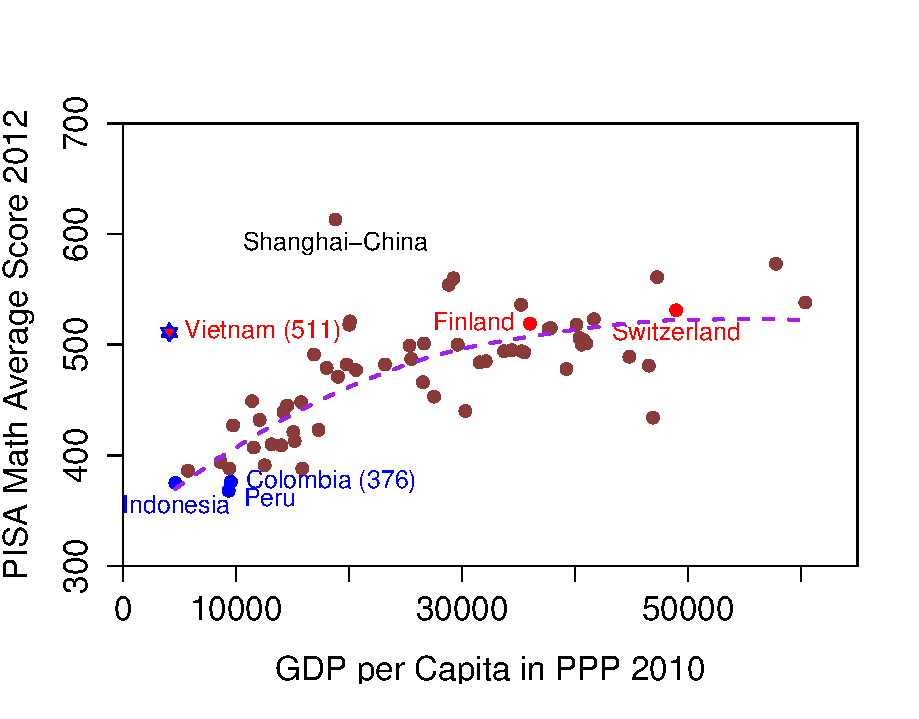
\includegraphics[width=0.75 \textwidth]{INTRFIG1.pdf} \\
\scriptsize{Source:OECD-PISA database        \hspace{3in}     }
   \label{Figure 1} 
\end{figure}

In the OECD-PISA database, there are seven countries other than Vietnam with a per capita GDP (in PPP dollars) below US\$ 10,000 - Albania, Colombia, Indonesia, Jordan, Peru, Thailand and Tunisia.  Their collective weighted average performance in mathematics was a mean score of 383. It is helpful to understand the significance of the 128 point difference with Vietnam. According to a recent OECD publication (\cite{OECD2013a}) \emph{``An entire proficiency level in mathematics spans about 70 score points \textendash  
a large difference in the skills and
knowledge students at that level possess. Such a gap represents the equivalent of about two years of schooling in the typical OECD country.''} Applying this heuristic would imply a nearly 3 year difference in attainment between Vietnam and the group of 7 developing countries in the PISA database. It should be noted at the outset that cross-section data from one instalment of PISA does not permit causal inference, but correlations can still provide useful insights. The difference is not only for mathematics and not just in the mean score, but spanning the entire test distribution, as can be seen in Figure 2.

\begin{figure}[H]
\caption{\textbf{Kernel Density comparison between Vietnam and other Developing Countries}}\label{fig:Kernel}
         \centering
         \begin{subfigure}[b]{0.3\textwidth}
                 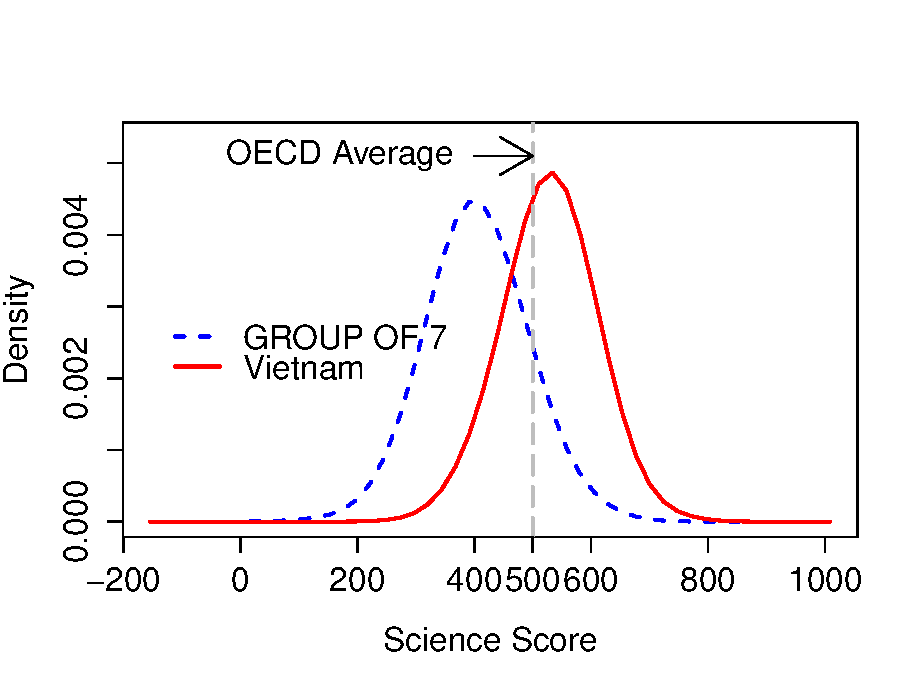
\includegraphics[width=\textwidth]{INTRFIG2a.pdf}
                 \caption{Science}
                 \label{fig:science}
         \end{subfigure}%
         ~ %add desired spacing between images, e. g. ~, \quad, \qquad, \hfill etc.
           %(or a blank line to force the subfigure onto a new line)
         \begin{subfigure}[b]{0.3\textwidth}
                 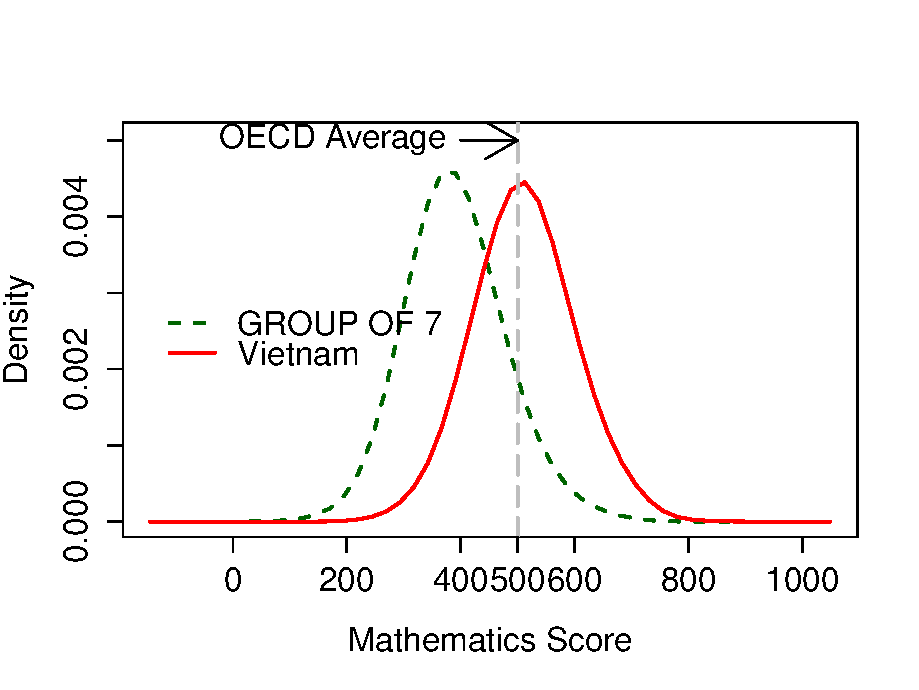
\includegraphics[width=\textwidth]{INTRFIG2b.pdf}
                 \caption{Mathematics}
                 \label{fig:mathematics}
         \end{subfigure}
         ~ %add desired spacing between images, e. g. ~, \quad, \qquad, \hfill etc.
           %(or a blank line to force the subfigure onto a new line)
         \begin{subfigure}[b]{0.28\textwidth}
                 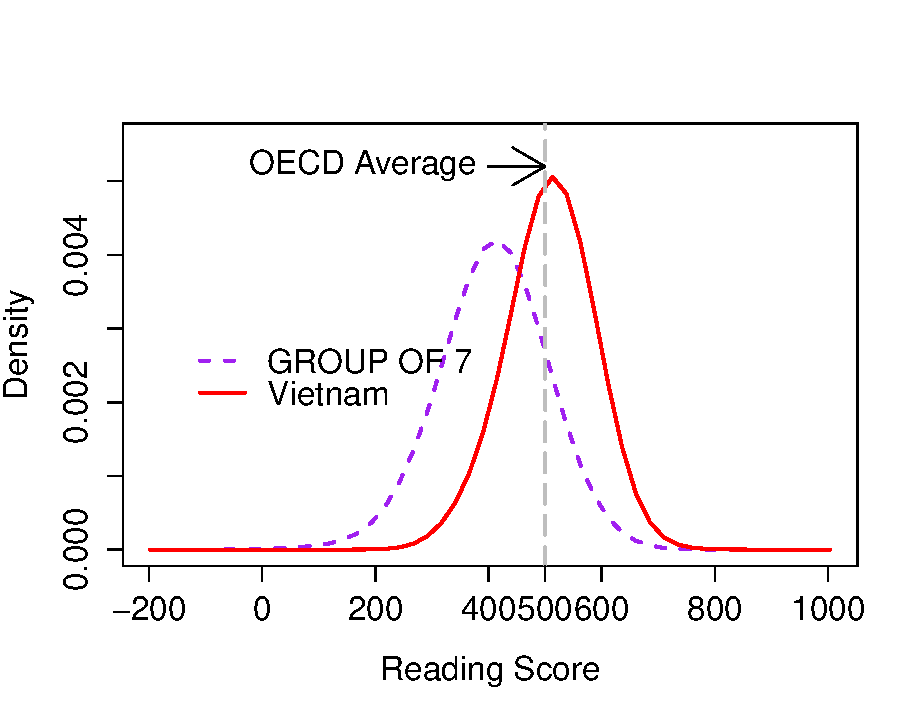
\includegraphics[width=\textwidth]{INTRFIG2c.pdf}
                 \caption{Reading}
                 \label{fig:reading}
         \end{subfigure}
     \end{figure}

A range of alternative classifications are possible to organize the possible explanatory factors available in the OECD-PISA database. Figure 3 presents four sets of factors, starting clockwise from the right. This is admittedly an arbitrary classification, utilized merely for expository purposes as we consider each of the constituent variables in turn. 

\begin{figure}[H]
   \caption{\textbf{Conceptual Scheme based on available comparative variables}}
   \centering 
     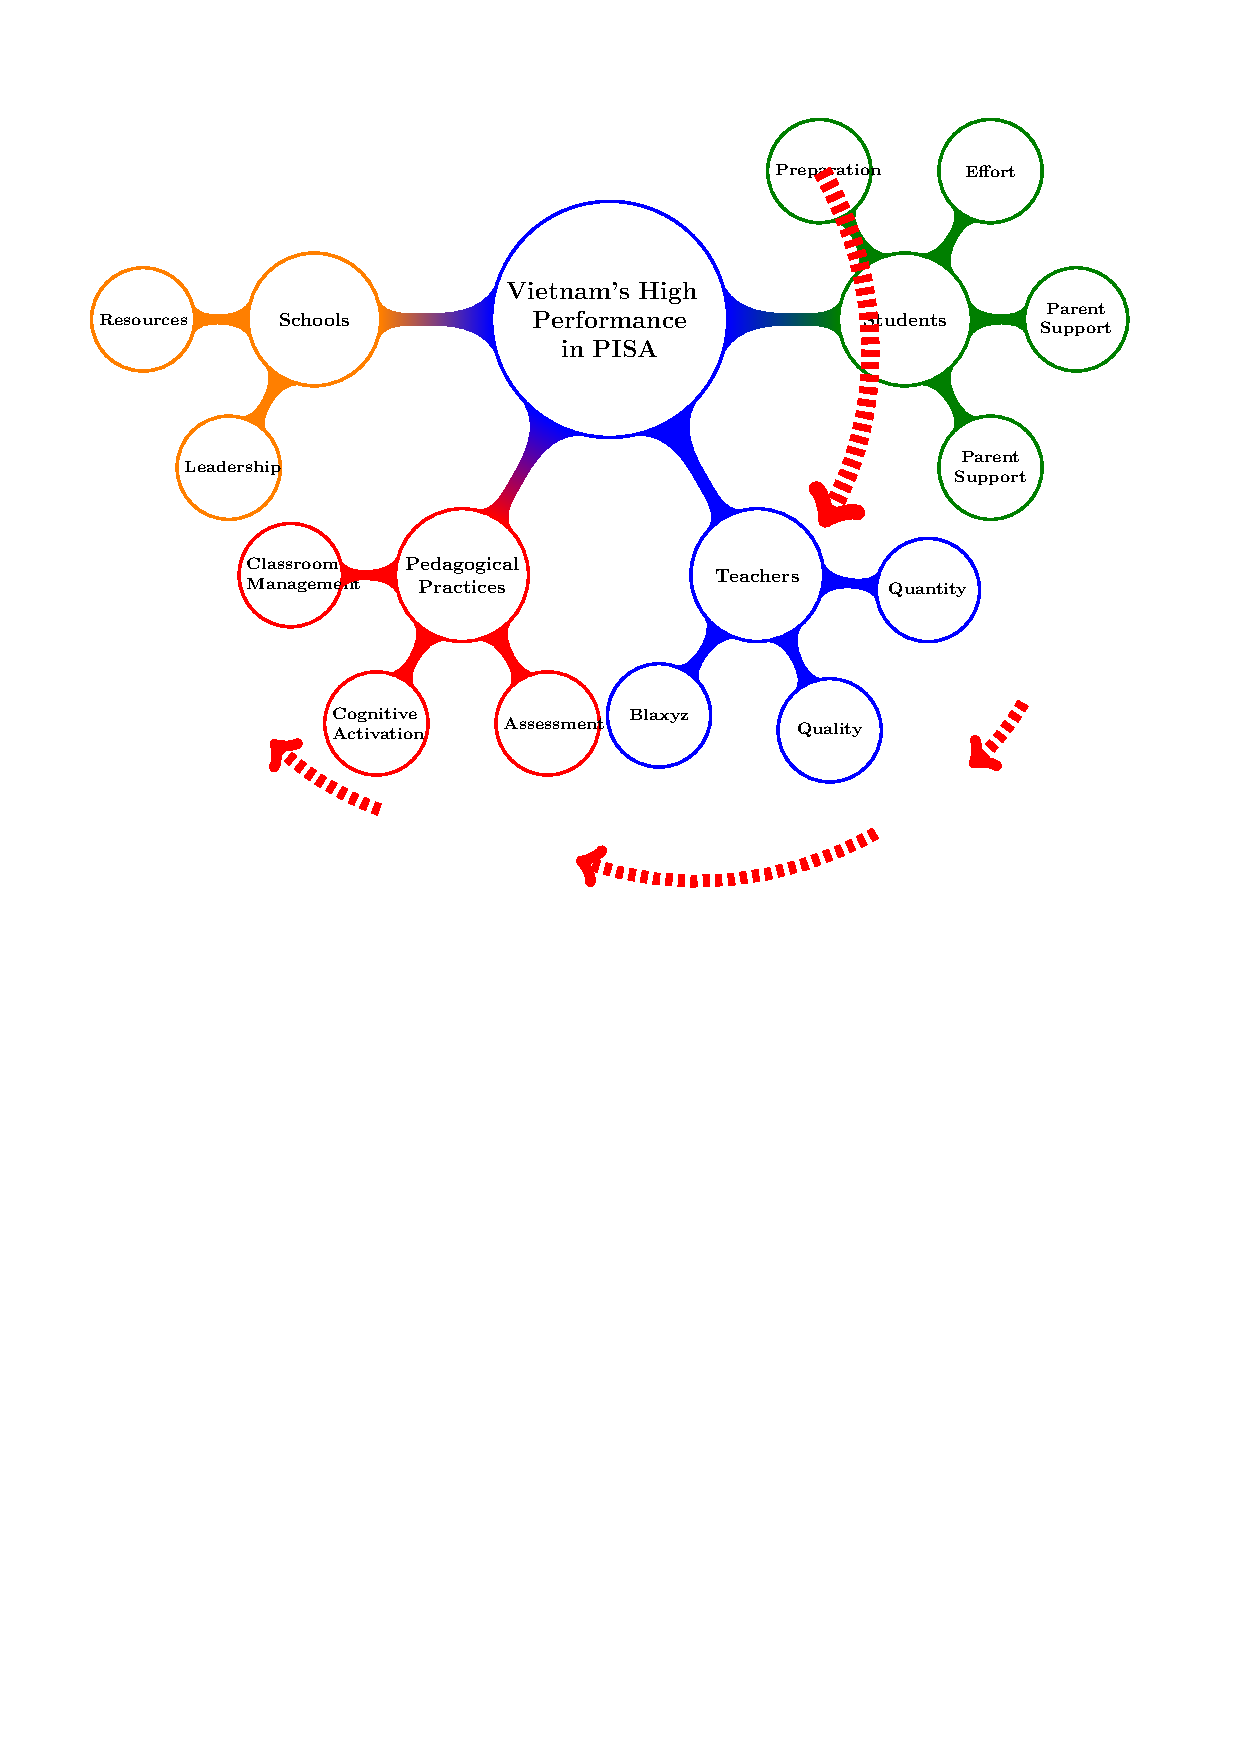
\includegraphics[width= 5in]{INTRTIKZ.pdf} \\
   \label{fig:m} 
\end{figure}

The approach of this paper is as follows. We begin in Section 2 by examining closely the differences in endowments between Vietnam and the collective group of 7 developing countries, termed as Dev7 for this paper (not to be confused with the G-7 of wealthy countries). The word `endowments' is used in a general sense, referring not merely to wealth related variables such as school resources, but to the range of policy, attitudinal and reported practices in the PISA dataset. The variables can also be considered as exogenous variables for the purpose of this analysis - in the first section we examine the mean differences in the levels of these variables. Comparing means in this context is a first pass at understanding the performance anomaly of Vietnam on empirical grounds. Without any priors, we want to look at seemingly obvious possible explanation - that Vietnamese 15 year olds somehow enjoy better endowments - economic, social, cultural and so on. This first pass can be quite revealing. For instance, even though we know that Vietnam's GDP per capita is the lowest in this G8 group of countries, perhaps the Vietnamese government and people have invested heavily in basic education, and schools in Vietnam enjoy much higher quality of facilities and equipment. Or the teachers have much higher level of education, and so on. Alternatively, one could find empirically that the schools are worse equipped and the teachers poorly trained. An examination of mean differences will provide us with a first set of tentative hypotheses.
\par
We make a second closer approach in Section 3 by adopting the regression methodology used by Fryer and Levitt in understanding differences in test score results of black children in the United States \cite{FryerLevitt04}. Differences in mean values of endowments leave some questions unanswered, which further analytical approaches can seek to resolve. In a multi-variate setting, we can try to understand how much of the variation can be explained by differences in observable endowments, and how much can be attributed to effects other than the observable differences. Fryer and Levitt have quite successfully followed the approach to explain what they see as evidence of a systemic difference in schools attended by black children. We adopt a similar approach to find out how much of the 'Vietnam gap' could reasonably be attributed to the earlier differences in mean endowments. As a matter of fact, we show in this section that the large differences in mean endowments is important, but it explains at best only half of the test score differences. 

The Fryer and Levitt method deepens the understanding from mean comparisons, but what it does not reveal may be as interesting as what it does reveal. Our Fryer-Levitt adaption is based on a pooled regression of eight developing countries, where we follow the fate of the magnitude of the coefficient of the dummy variable representing the Vietnamese student in the sample.  But we also need to investigate structural differences in the effects of endowments between Vietnam and Dev7 countries. In Section 4, we adopt an approach first used to explain variation in PISA performance between Germany and Finland by Andreas Ammermueller \cite{Ammermueller07}. This is an adaptation of the popular Oaxaca-Blinder decomposition of wage earnings equation to uncover evidence of discrimination on the basis of gender. \cite{Blinder73} and \cite{Oaxaca73} In this section, we can examine closely the structural differences between Vietnam and the Dev7 countries, including the contribution of differences in endowments and the coefficients to the gap in test scores. 

Even a multi-variate regression approach only proves correlation with nothing more than a hint regarding causation, and so far we have only one year (2012) of PISA data for Vietnam. PISA 2015 data will be available in 2016 and analytical approaches closer to establishing causality can be attempted. Even with the caveat regarding causality, there are useful policy related conclusions that we can derive from the analysis presented in this paper - learning for Vietnam, with regard to areas of strengths and weaknesses; and learning for other countries that may wish to emulate aspects of Vietnam's performance. There is a veritable industry of papers regarding Finland's PISA performance, directed mostly towards other OECD countries with lower scores, for instance United States. Vietnam's superlative performance points to a similar future stream of research, with the added advantage of relevance for developing countries. Section 5 provides concluding ideas that might be amongst the first of many more such ideas from future investigations of Vietnam's performance. 


\section{Endowment Differences regarding Student, Family, Teachers and Schools}

\subsection{Student Characteristics}

Table 1 begins an exploration of differences in mean values between Vietnam and Dev7 students. This exploration only provides us with a beginning in our task of unravelling the mystery of Vietnam's performance. Neither mean differences nor the regressions that follow can claim to uncover causality. However, they do provide what in a court of law could be called `circumstantial evidence'. Table 1 presents student characteristics, and it should be noted that the absence of differences is sometimes as important as the presence of differences. Table 1 indicates no differences by age or gender of student.  The PRESCHOOL variable shows the first instance of a statistically siginificant difference. While 78.88\% of Dev7 students reported attending preschool, the number of students attending preschool from the Vietnam sample was 91.20\% - a sizeable difference both statistically and economically significant. The relationship between preschool and later outcomes has been studied very closely over the years. Longitudinal impact evaluation studies regarding the Perry Preschool project and Head Start in the US are amongst the most cited studies in the economics literature\footnote{For detailed meta-analysis, see \cite{Barnett95} and \cite{Schweinhartetal05}}. We can also see from the numbers for REPEAT in Table 1 that PISA takers in Vietnam were three times less likely to have repeated a grade in the past (6.79\% compared to 19.15\%).

\begin{table}[H]
	\tiny
	\def\arraystretch{0.9}
	\centering
	\caption{\textbf{Student characteristics and family background}}
	\begin{tabulary}{1.0\textwidth}{L L C C C C}
		\hline\hline \\
		\multicolumn{2}{c}{}
		& \multicolumn{2}{c}{Dev7 countries}
		& \multicolumn{2}{c}{Vietnam}	\\
		\hline & & & & & & 
		Variable & Description & MS & Valid N &  MS & Valid N \\
		\hline \\
		\multicolumn{6}{l}{\textbf{Fixed characteristics}}	\\ [0.3em]
      \hline \\
		FEMALE & Sex of student & 0.5265 & 41394 & 0.5336 & 4882 \\ 
		& & (0.4993) &  & (0.4989) &  \\ [0.3em]
      AGE & Age of student & 15.8211 & 41394 & 15.7692 & 4853 \\ 
		& & (0.2895) &  & (0.2885) &  \\ [0.3em]
     \hline \\
     \multicolumn{6}{l}{\textbf{Student's prior history}}	\\ [0.3em]
     \hline \\ 
		PRESCHOOL & Attended Preschool & 0.7888 & 40114 & 0.912 & 4866 \\ 
		&  & (0.4082) &  & (0.2833) &  \\ 
		REPEAT & Grade repeating & 0.1915 & 40343 & 0.0679 & 4860 \\ 
		& &  (0.3935) &  & (0.2516) &  \\ [0.3em]
     \hline \\
     \multicolumn{6}{l}{\textbf{Truancy from School}}	\\ [0.3em]
     \hline \\ 
		ST08Q01 & Times late & 1.5131 & 40663 & 1.1872 & 4873 \\ 
		& for school & (0.7648) &  & (0.4685) &  \\ [0.3em]
		ST09Q01 & Days unexcused & 1.2192 & 40650 & 1.0999 & 4875 \\ 
		& absence & (0.5276) &  & (0.3527) &  \\ [0.3em]
		ST115Q01 & Times skipped & 1.2585 & 40632 & 1.0764 & 4880 \\ 
		& classes & (0.545) &  & (0.3216) &  \\ [0.3em]
     \hline \\
     \multicolumn{6}{l}{\textbf{Parental background and family wealth}}	\\ [0.3em]
     \hline \\ 
		HISEI & Highest parental & 40.4196 & 32814  & 26.6023 & 4860 \\ 
		& occupational status & (22.5168) &  & (19.855) &  \\ [0.3em]
		MISCED & Educational level & 3.1193 & 40486 & 2.1744 & 4844 \\ 
		& of mother (ISCED) & (1.9853) &  & (1.6059) &  \\ [0.3em]
		WEALTH & Family wealth & -1.4606 & 40821 & -2.1343 & 4881 \\ 
		& possessions & (1.2267) &  & (1.1656) &  \\ [0.3em]
		CULTPOS & Cultural possessions & -0.1424 & 39905 & -0.2361 & 4809 \\ 
		& & (0.9678) &  & (1.0173) &  \\ [0.3em]
		HEDRES & Home educational &  -0.7427 & 40579 & -1.0743 & 4874 \\ 
		& resources & (1.1473) &  & (0.9364) &  \\ [0.3em]
		BOOK\_N & Number of books & 53.6393 & 39631 & 50.786 & 4841 \\ 
		& in family home & (94.5556) &  & (75.4031) &  \\[0.3em]
		\hline \\
	\multicolumn{6}{l}{Notes: The variables relate to the questionnaires administered to students in the general}\\    
	\multicolumn{6}{l}{(non-rotated) booklet. For a more detailed description of variables, please see Table xx.}\\
	\multicolumn{6}{l}{Items marked with \textit{(r)} are taken from the rotated student questionnaire. The variable}\\
	\multicolumn{6}{l}{means of Dev7 and Vietnam are statistically different at the 95\% significance level, except}\\
	\multicolumn{6}{l}{FEMALE.}\\
\end{tabulary}
\end{table}
The finding regarding PRESCHOOL and REPEAT indicates the possible importance of the trajectory of the student prior to High School. Repetition rates are difficult as comparative indicators of system quality because of the variations across countries in curriculum and standards, but REPEAT is another interesting variable to keep in mind as a possible clue to the mystery of Vietnam's PISA performance. As in some other East Asian cultures, Vietnamese children are expected by their parents to study hard. Though Mark Twain in Vietnamese translation is quite a best seller for young readers in Vietnam, truancy from school is not perceived benovelently by parents.\footnote{A cultural explanation is possibly quite important in explaining Vietnam's anomalous PISA results, though the PISA dataset may only be able to measure the possible effects of culture rather than measuring cultural differences. Literature from the World Values Survey, that does seek to measure cultural differences, indicates that Vietnam is a positive outlier on discipline and authority orientation\cite{DaltonOng05}.} Table 1 indicates a consistently lower truancy rate for the three variables used - the question refers to the past week \textbf{(to confirm)} and Vietnamese students are less likely to be late for school, have fewer days of unexcused absence and skip fewer classes.\footnote{In the student's questionnaire, there is a telling question - student's have to agree or disagree on a four point Likert scale to the statement ``If I had different teachers, I would try harder at school.''. Converted into an index, the mean for Vietnam at 0.363 is lower than that for Dev7 at 0.525. This suggests a tendency in Vietnamese students for greater self-responsibility.} 

The final set of variables in Table 1 concern parental background and wealth at the students home, including cultural resources and books at home which may work to stimulate cognitive development. The PISA database includes a number of indices to measure aspects such as weath and possessions. These indices are based on underlying data regarding occupations and possessions. The scaling of raw data to indices is described in detail in the PISA technical report \cite{OECD2014a}. For HISEI, the parents occupation status, the OECD mean is 50 and the OECD standard deviation is 15. Table 1 shows that the HISEI for Dev7 parents at 40.42 was much higher than 26.60 for Vietnamese parents. MISCED refers to the International Standard Classification of Education (ISCED) developed by UNESCO. Table 1 shows that the average level of mother's education for Dev7 was just over 3, meaning Upper Secondary education, while for Vietnam the mean was just over 2, meaning Lower Secondary education. The WEALTH index is set for an OECD mean of zero and standard deviation of 1. Dev 7 countries wealth level was -1.5 and Vietnam's was -2.1, consistent with the data regarding occupational classification and mother's education. These findings indicate the close correlation of these variables with GDP per capita. The more interesting finding concerns the indices CULTPOS and HEDRES, which have OECD mean 0 and s.d. 1, and the number of books. CULTPOS includes classical literature, books of poetry and works of art. HEDRES includes reference books and books to help with school work as well as a study desk and 'a quiet place to study'. These three variables are also in line with per capita income - with the Dev7 mean being lower than the OECD mean, and Vietname being lower than Dev7. So one explanation regarding Vietnam's PISA performance can probably be ruled out - it does not seem likely that Vietnamese households spend disproportionately higher amount of their incomes on acquiring possessions that would give their children an edge in life. Books and other education related articles are owned by Vietnamese households to the same extent as any other households. 

\subsection{Student Effort}

The phenomenon of primary and high school children taking extra classes to supplement in school instruction in Vietnam is well known \cite{HaHapharm05} and \cite{Hai-Anh07}. Table 2 indicates that while Dev7 students spent roughly 4.7 hours in such classes (total of OUTMATH, OUTLANG and OUTSCIE), the Vietnamese student spent nearly 2 hours more for a total of 6.6 hours, with the difference being highest for OUTMATH. Vietnamese students also spent about 1 additional hour per week doing homework (total of ST57Q01 and ST57Q02) compared to Dev7 students. The highest difference in this set of variables concerns the variable ST57Q04, which relates to extra classes taught by a commercial company. While most of the schools in Vietnam are public or government schools, it is interesting to note that students report nearly 5 hours of commercially provided extra lessons, while the total for Dev7 countries is only about 2 hours. Collectively, these variables indicate that Vietnamese students spent about 16 hours per week studying outside of school, compared to 13 hours per week for Dev7 students. 

\begin{table}[H]
	\tiny
	\def\arraystretch{0.9}
	\centering
	\caption{\textbf{Student studying time out of school}}
	\begin{tabulary}{1.0\textwidth}{L L C C C C}
		\hline\hline \\
		\multicolumn{2}{c}{}
		& \multicolumn{2}{c}{Dev7 countries}
		& \multicolumn{2}{c}{Vietnam}	\\
		\hline & & & & & & 
		Variable & Description & MS & Valid N &  MS & Valid N \\
		\hline \\
\multicolumn{6}{l}{\textbf{Weekly out-of-school hours per subject}}	\\ [0.3em]
\hline \\
OUTMATH & weekly out-of-school & 1.828 & 23603 & 3.1305 & 3227 \\ 
& lessons in math & (2.1539) &  & (2.3133) &  \\ [0.3em]
OUTREAD & weekly out-of-school & 1.2882 & 23531 & 1.4483 & 3223 \\ 
& lessons in 'test language'& (1.9623) &  & (1.8837) &  \\ [0.3em]
OUTSCIE & weekly out-of-school & 1.5609 & 23298 & 2.0927 & 3205 \\ 
& lessons in science & (2.0456) &  & (2.1776) &  \\ [0.3em]
\hline \\
\multicolumn{6}{l}{\textbf{Weekly out-of-school hours approach}}	\\ [0.3em]
\hline \\
ST57Q01 \textit{(r)} & Out-of-school time & 5.0953 & 23696 & 5.8145 & 3164 \\ 
& homework & (5.0319) &  & (5.7196) &  \\ [0.3em]
ST57Q02 \textit{(r)} & Out-of-school time & 2.551 & 19355 & 2.8814 & 2285 \\ 
& guided homework & (2.9296) &  & (3.2384) &  \\ [0.3em]
ST57Q03 \textit{(r)} & Out-of-school time & 1.7276 & 20367 & 1.5749 & 3049 \\ 
& personal tutor & (2.7884) &  & (2.938) &  \\[0.3em]
ST57Q04 \textit{(r)} & Out-of-school time & 1.892 & 19517 & 4.878 & 3091 \\ 
& classes by company & (3.3487) &  & (4.8058) &  \\ [0.3em]
ST57Q05 \textit{(r)} & Out-of-school time & 2.1354 & 21542 & 1.7646 & 3092 \\ 
& parent/family member & (3.055) &  & (3.2442) &  \\ [0.3em]
ST57Q06 \textit{(r)} & Out-of-school time & 2.588 & 21338 & 1.8029 & 3079 \\ 
& learn on computer & (3.5519) &  & (3.0496) &  \\ [0.3em]
		\hline \\
		\multicolumn{6}{l}{Notes: The variables relate to the questionnaires administered to students in the rotated booklet.}\\   
		\multicolumn{6}{l}{For a more detailed description of variables, please see Table xx. Items marked with \textit{(r)} are}\\    
		\multicolumn{6}{l}{taken from the rotated student questionnaire. The variable means of Dev7 and Vietnam are}\\
		\multicolumn{6}{l}{statistically different at the 95\% significance level.}\\		
	\end{tabulary}
\end{table}

\subsection{Student Attitudes}

PISA applications in each round have a focus on one of the subjects and in PISA 2012 the focus subject was mathematics. Mathematics happens to be the subject where the score difference is highest between Vietnam and Dev7 countries. The PISA questionnaire for students includes a very interesting series of questions regarding student's perceptions of their abilities, their effort and their reported practices. The details of these questions can be found in the PISA Technical Manual. Typically, each question includes a set of likert scaled items to which the student provides a discrete response on a four point agree-disagree scale. These responses then are combined under specified algorithms to provide an index value. For instance, there is a question to which the response is meant to measure a student's MATWKETH or `mathematics work ethic'. Students either agree or disagree with a set of 9 items on a 4 point likert scale - strongly disagree, disagree, agree and strongly disagree. The items include items such as ``I work hard on my mathematics homework'',  and ``I listen in mathematics class'', ``I keep my mathematics work well organized''. In the case of this example, when a student agrees or strongly agrees with a positive statement, or disagrees/strongly disagrees with a negative statement, he or she would tend to be deemed to have a stronger work ethic towards mathematics. The raw data from the likert scale is converted into an index using IRT scaling procedures, so that the mean for OECD countries is 0 and standard deviation is 1. Table 3 indicates a most interesting finding regarding a range of such indices from the PISA database.

\begin{table}[H]
	\tiny
	\def\arraystretch{0.9}
	\centering
	\caption{\textbf{Student self-perception regarding mathematical ability and student effort}}
	\begin{tabulary}{1.0\textwidth}{L L C C C C}
		\hline\hline \\
		\multicolumn{2}{c}{}
		& \multicolumn{2}{c}{Dev7 countries}
		& \multicolumn{2}{c}{Vietnam}	\\
		\hline & & & & & & 
		Variable & Description & MS & Valid N &  MS & Valid N \\
		\hline \\
	\multicolumn{6}{l}{\textbf{Indices susceptible to 'bragging' tag }}	\\ [0.3em]
	\hline \\		
   MATWKETH \textit{(r)} & Mathematics & 0.4514 & 26140 & -0.0014 & 3217 \\ 
	& work ethic & (0.9782) &  & (0.6915) &  \\ [0.3em]	
	SUBNORM \textit{(r)} & Subjective norms & 0.716 & 26509 & -0.0923 & 3220 \\ 
	& in mathematics & (1.165) &  & (0.8395) &  \\ [0.3em]
	OPENPS \textit{(r)} & Openness to & 0.1949 & 25612 & -0.6125 & 3207 \\ 
	& problem solving & (0.9787) &  & (0.8708) &  \\ [0.3em]
	SCMAT \textit{(r)} & Self-concept of & 0.1673 & 26222 & -0.1896 & 3249 \\ 
	&  own math skills & (0.8101) &  & (0.5903) &  \\ [0.3em]
	\multicolumn{6}{l}{\textbf{Indices less related to being modest/boastful}}	\\ [0.3em]
	\hline \\		
	PERSEV \textit{(r)} & Perseverance & 0.3387 & 25710 & 0.4475 & 3211 \\ 
	& in problem solving & (0.9605) &  & (0.8767) &  \\ [0.3em]
	ANXMAT \textit{(r)} & Mathematics & 0.3995 & 26275 & 0.2115 & 3248 \\ 
	& Anxiety & (0.7724) &  & (0.6354) &  \\ [0.3em]
	MATINTFC \textit{(r)} & Mathematics & 0.092 & 24827 & 0.3285 & 3181 \\ 
	& intentions & (0.9837) &  & (1.0964) &  \\ [0.3em]
		\hline \\
		\multicolumn{6}{l}{Notes: For the full set of results, please consult the github repository for this paper}\\	
\end{tabulary}
\end{table}

The upper panel in Table 3 indicates a set of indices where the scores for  Vietnamese students are lower than the scores for Dev7 students. For example, the score for MATWKETH is 0.45 for Dev7 and 0 for Vietnam. The variable SUBNORM is supposed to measure subjective norms regarding mathematics. This construct relates to a student's perceptions regarding how other people in the student's life value mathematics. It includes items such as ``my friends enjoy taking mathematics tests'' and ``my parents believe it's important for me to study mathematics.'' Presumably, when this measure is high, the student has a high subjective norm for mathematics. Table 3 shows the resulting mean for Dev7 countries is 0.72 and the value for Vietnam is -0.09. The index SCMAT includes items such as ``I learn mathematics quickly'' and ``I have always believed that mathematics is one of my best subjects''. Vietnamese students, who scored more than 1 standard deviation above the Dev7 students on the PISA math test, scored half a standard deviation lower on SCMAT. What is going on here ?

This mini-mystery within the overall mystery can possibly be resolved by looking at all the indices. There was a set of indices  with low performance difference between Dev7 and Vietnam and they do not shed much light on the seemingly contradictory result reported in the upper panel on Table 3. The lower panel of Table 3 reports on indices where the balance tips on the other side - these are indices where Vietnamese students performed better than the Dev7 students. The three indices here bear close examination. PERSEV consists of items that purport to capture perseverance with a task or a problem to resolve; ANXMAT is a negative index (less is better) that deals with mathematics anxiety (for example an item is ``I get very nervous doing mathematics problems''); MATINTFC relates to future mathematics intention, including items such as ``I am planning on majoring in a subject in college that requires lot of mathematics''. 

One possible explanation, as indicated in the heading of the Table 3 panels, is that Vietnamese students are bought up in a culture that stresses the importance of modesty and humility as a pathway to learning. They may find it difficult to say great things about themselves, because of cultural norms against bragging or boasting. The lower panel in Table 3, on the other hand includes items that are less prone for an immodest interpretation. To say that you are not afraid of mathematics may not be perceived as bragging. And in this context, the Vietnamese students are less anxious and more confident about the the future of mathematics in their life.\footnote{It will be straightforward to examine this hypothesis more closely by performing an IRT scaling of the underlying items for the indices. We can then test for differences between Vietnam and the Dev7 countries in values of the  location parameters linking the items to the index. Systematic differences will tend to support the hypothesis laid out here.}

\subsection{Mathematics Curriculum}

In addition to beliefs and perceptions of students regarding mathematics in general, PISA also seeks to investigate more closely the issue of content of mathematics instruction. PISA incorporates a very interesting approach to avoid or minimize the bragging or over-claiming problem referred to in the previous sub-section. The index FAMCON is constructed out of a response to a question about mathematical concepts for which students are asked ``How familiar are you with the following items?'' The list of items includes items such as `Linear Equation', `Quadratic Function'  and `Cosine.' The list of items also includes three nonsensical items or pseudo-concepts that sound fancy: `Proper Number',`Subjunctive Scaling' and Declarative Fraction'. These items are termed as FOIL, and are used as trick items to calibrate the response for over-claiming on part of the students. The index without correction is presented as FAMCON, and the index with correction is presented as FAMCONC. It is quite fascinating that with FAMCON, the uncorrected version, Dev7 students come out apparently better than Vietnam students mean of 0.26 as compared to 0.12. Unfortunately, it appears that this also included familiarity with non-existent items like `subjunctive scaling' - or bragging. With the corrected version, FAMCONC, the Vietnamese students turn out to do much better, with a mean value of 0.43 as compared to Dev7 mean of -0.54. 

\begin{table}[H]
	\tiny
	\def\arraystretch{0.9}
	\centering
	\caption{\textbf{Student reported experience in mathematics}}
	\begin{tabulary}{1.0\textwidth}{L L C C C C}
		\hline\hline \\
		\multicolumn{2}{c}{}
		& \multicolumn{2}{c}{Dev7 countries}
		& \multicolumn{2}{c}{Vietnam}	\\
		\hline & & & & & & 
		Variable & Description & MS & Valid N &  MS & Valid N \\
		\hline \\	
		FAMCON \textit{(r)} & Familiarity with & 0.2559 & 26164 & 0.1225 & 3243 \\ 
		& math concepts & (1.1654) &  & (0.6935) &  \\ 	[0.3em]
		FAMCONC \textit{(r)} & FAMCON corrected & -0.5441 & 25832 & 0.4297 & 3231 \\ 
		& with FOIL & (0.8768) &  & (0.9057) &  \\ 	[0.3em]
		EXAPPLM \textit{(r)} & Experience with & 0.1111 & 26133 & -0.2418 & 3243 \\ 
		& applied math tasks & (1.06) &  & (0.7624) &  \\ [0.3em]
		EXPUREM \textit{(r)} & Experience with pure & -0.1384 & 25973 & 0.1587 & 3244 \\ 
		& math tasks & (0.9809) &  & (0.8076) &  \\ [0.3em]
		\hline \\
		\multicolumn{6}{l}{Notes: The variables relate to the questionnaires administered to students in the rotated}\\   
		\multicolumn{6}{l}{booklet. For a more detailed description of variables, please see Table xx. Items marked}\\    
		\multicolumn{6}{l}{with \textit{(r)} are taken from the rotated student questionnaire. The variable means of}\\
		\multicolumn{6}{l}{Dev7 and Vietnam are statistically different at the 5\% significance level.}\\
\end{tabulary}
\end{table}

The index EXAPPLM asks students about their experience during school work with examples of applied mathematics problems. Similarily, the index EXPUEM refers to experience with examples of pure mathematics. Not surprisingly, Vietnam students indicate a lower performance on EXAPPLM and a higher performance on EXPUREM.\footnote{It has been a long standing issue that Vietnamese students are expected to learn a curriculum that is more crammed than the international norm, but has more of theory and abstract mathematics rather than applied mathematics.See \cite{NguyenTran13} and \cite{Le07}.} To the extent that the PISA mathematics test almost by definition tends towards pure rather than applications in real life, the figures help to understand Vietnam's performance.

\subsection{Parental Support at School} 

The publication of the bestseller book \cite{Chua11} ``Battle Hymn of the Tiger Mother'' in 2011 ignited a firestorm of controversy. The book gave prominence in the popular culture to a vast academic literature regarding parenting styles and about the perceived higher performance of children from Asian immigrant families in the US and other western countries.One of the ways that parents influence children's education outcome is through the interaction that parents have with their child's teachers and others at school. The PISA data includes a question that asks about parental expectations.This question (SC24) includes a statement ``There is \emph{constant pressure} from many parents, who expect our school to set very high academic standards and to have our students achieve them.'' The\footnote{\cite{HsienXie14} investigate in detail the data from a set of longitudinal surveys that cover thousands of children over a long period starting from their early childhood through high school. As part of the explanation of the superior performance of Asian immigrant children, the authors report that ``Asian students report greater parental expectations of academic success.'' }  Table 4 indicates a higher level of PARPRESSURE for Vietnam as compared to Dev7.  Another question (SC25) asks school principals about the proportion of parents that take part in a set of 12 activities. While the question does not specify which parent (or both) may be involved, the variables have been named after the mother for ease of exposition. 

\begin{table}[H]
	\tiny
	\def\arraystretch{0.9}
	\centering
	\caption{\textbf{Parental Support at School}}
	\begin{tabulary}{1.0\textwidth}{L L C C C C}
		\hline\hline \\
		\multicolumn{2}{c}{}
		& \multicolumn{2}{c}{Dev7 countries}
		& \multicolumn{2}{c}{Vietnam}	\\
		\hline & & & & & & 
		Variable & Description & MS & Valid N &  MS & Valid N \\
		\hline \\
		PARPRESSURE & Parental achievement & 0.2665 & 40372 & 0.3837 & 4866 \\ 
		& pressure & (0.4421) &  & (0.4863) &  \\  [0.3em]
		TIGERMOM & Parent initiates - &  52.4472 & 41394 & 62.4183 & 4882 \\ 
		& progress discussion & (38.097) &  & (41.3743) &  \\ [0.3em]
		DUTYMOM & Teacher initiates - &  66.9737 & 41394 & 68.5543 & 4882 \\ 
		& progress discussion & (36.727) &  & (37.4796) &  \\ [0.3em]
		VOLUMOM & Parent Participation - & 35.2134 & 41394 & 38.3623 & 4882 \\ 
		& Volunteering & (38.8428) &  & (39.9773) &  \\ [0.3em]
		TEACHMOM & Parent Participation - & 12.1764 & 41394 & 38.2821 & 4882 \\ 
		& Teaching Assistance & (23.4241) &  & (41.5357) &  \\ [0.3em]
		FUNDMOM & Parent Participation - & 23.0784 & 41394 & 59.6022 & 4882 \\ 
		& Fundraising & (35.2134) &  & (44.0376) &  \\ [0.3em]
		COUNCILMOM & Parent Participation - & 36.4546 & 41394 & 23.1174 & 4882 \\ 
		& School government & (37.2252) &  & (36.4406) &  \\[0.3em]
		\hline \\
		\multicolumn{6}{l}{Notes: The variables relate to the questionnaires administered to students in the rotated booklet}\\   
		\multicolumn{6}{l}{and the general (non-rotated) booklet. For a more detailed description of variables, please see}\\    
		\multicolumn{6}{l}{Table xx. Items marked with \textit{(r)} are taken from the rotated student questionnaire. The variable}\\
		\multicolumn{6}{l}{means of Dev7 and Vietnam are statistically different at the 5\% significance level.}\\	
	\end{tabulary}
	\end{table}

TIGERMOM refers to the reported proportion of parents who discussed their child's behavior or the child's progress ``on their own initiative'', to differentiate from cases where parents might have done so on the initiative of the teacher, termed as DUTYMOM. Table 4 shows a slightly higher number on DUTYMOM for Vietnamese parents compared to Dev7, but a greater difference, more than ten percentage points for TIGERMOM. VOLUMOM refers to parents volunteering in various non-academic activities, such as field trips or carpentry and yard work. Vietnamese parents appear to have slight advantage with regard to VOLUMOM, buta much  higher advantage when considering TEACHMOM, which refers to parents volunteering as assistants to the teacher - 12.18\% compared to 38.28\%. Vietnamese parents also appear to be much more active in fund raising, from the values for FUNDMOM, though they may have less formal influence through school committees. 

\subsection{Teacher Characteristics} 

Conventional measures regarding student-teacher ratio and teacher certification show some advantage for Vietnam over Dev7 as shown in Table 6.  

\begin{table}[H]
	\tiny
	\def\arraystretch{0.9}
	\centering
	\caption{\textbf{Teacher characteristics and management}}
	\begin{tabulary}{1.0\textwidth}{L L C C C C}
		\hline\hline \\
		\multicolumn{2}{c}{}
		& \multicolumn{2}{c}{Dev7 countries}
		& \multicolumn{2}{c}{Vietnam}	\\
		\hline & & & & & & 
		Variable & Description & MS & Valid N &  MS & Valid N \\
		\hline \\
		\multicolumn{6}{l}{\textbf{Teacher numbers and teacher management}}	\\ [0.3em]
		\hline \\ 
		PROPCERT & Proportion of & 0.6757 & 35130 & 0.7961 & 4586 \\ 
		& certified teacher & (0.4042) &  & (0.3978) &  \\ [0.3em]
		SMRATIO & Mathematics & 188.1791 & 33985 & 120.9773 & 4777 \\ 
		& teacher-student ratio & (158.6256) &  & (43.6092) &  \\ [0.3em]
		SC35Q02 & Professional development & 40.5068 & 39550 & 49.0086 & 4762 \\ 
		& in math in last 3 months & (40.8546) &  & (45.1706) &  \\ [0.3em]
		& teaching style & (0.9613) &  & (0.774) &  \\ [0.3em]
		STUDREL \textit{(r)} & Teacher student & 0.3794 & 25870 & 0.0186 & 3253 \\ 
		& relations & (1.0178) &  & (0.8883) &  \\ [0.3em]
		TCH\_INCENTV & Teacher appraisal  &  -0.0317 & 41394 & 0.2687 & 4882 \\ 
		& linked to incentives & (1.0301) &  & (0.6336) &  \\ 	[0.3em]
		\hline \\
		\multicolumn{6}{l}{\textbf{Quality assurance of mathematics teachers through \ldots}}	\\ [0.3em]
		\hline \\ 
		TCH\_MENT & Teacher mentoring & 0.8566 & 40734 & 0.9859 & 4882 \\ 
		& as quality assurance & (0.3505) &  & (0.1181) &  \\ [0.3em]
		TCM\_PEER & Teacher peer review & 0.7916 & 41095 & 0.8382 & 4882 \\ 
		& of lectures, methods etc & (0.4061) &  & (0.3683) &  \\ [0.3em]
		TCM\_OBSER & Principal or senior & 0.8015 & 41170 & 0.9785 & 4882 \\ 
		& staff observations & (0.3989) &  & (0.1451) &  \\ [0.3em]
		TCM\_INSPE & Observation of classes & 0.5882 & 41020 & 0.8664 & 4882 \\ 
		& external inspector & (0.4922) &  & (0.3402) &  \\ [0.3em]
		\hline \\
		\multicolumn{6}{l}{Notes: The variables relate to the questionnaires administered to principals (schools) and}\\    
		\multicolumn{6}{l}{students in the rotated booklet. For a more detailed description of variables, please see}\\
	\end{tabulary}
	\end{table}

The student-teacher ratio overall is not much different at about 20 students per teacher, but there are more specialized mathematics teachers in Vietnam, as shown by the values for SMRATIO (121 in Vietnam compared to 188 for Dev7). There is a higher percentage of certified teachers in Vietnam, and higher reported professional development in mathematics (SC35Q02). A very interesting variable from a policy point of view regards incentives for teachers. School principals were questioned to what extent performance appraisal or other forms of feedback  are related to incentives for teachers in seven different forms, from salary and bonus to public recognition and greater job responsibilities. The answers were on a 4 point scale: `No change', `A small change', 'A moderate change' and 'A large change'. We converted the rating into a Rasch index, scaled to an OECD mean of 0 and standard deviation of 1. The mean for Dev7 for this index, TCH\_INCENTV was -0.03 for Dev7 and 0.27 for Vietnam, indicating greater presence of teacher incentives in Vietnam. The final set of variables in Table 6 deal with the way that quality assurance regarding teacher performance is carried out, with help of a mentor, peer, supervisor and external inspector. These variables indicate a higher prevalence of oversight for teachers in Vietnam, with the difference being greatest for external inspections (86.64\% in Vietnam compared to 58.82\% in Dev7 countries). 

\subsection{Pedagogical Practices} 

Pedaogical practices are an outcome of a complex interaction between curriculum and other policy, economic possibilities and the cultural and historical context. It is difficult to trace differences in these practices in a quantitative survey.\footnote{For an interesting recent qualitative study that seeks to emulate the TIMSS video study for Vietnam, see \cite{Phuong14}.} Table 7 presents a few variables that seek to capture variation in pedagogical practices. Table 7 indicates the higher prevalence of national policies in Vietnam regarding the use of computers in the classroom and the use of a standardized curriculum that specifies what has to be taught each month. There is no difference with regard to the use of a single textbook. There is some difference in the use of formative student assessment, with slightly higher percentage of use of assessments to monitor teachers and schools. COGACT is an OECD-PISA index variable based on response to student reports regarding classroom practices such as teacher requiring students to reflect on a problem or develop procedures rather than practice given procedures. This variables show much lower level of cognitive activation in Vietnam (-0.33) compared to 0.30 for Dev7. In the final set of classroom management variables, an interesting variation can be seen in DISCLIMA, an index variable that measures disciplinary climate in class, and is higher for Vietnam (0.38) as compared to Dev7 (-0.02).

\begin{table}[H]
	\tiny
	\def\arraystretch{0.9}
	\centering
	\caption{\textbf{Pedagogical practices}}
	\begin{tabulary}{1.0\textwidth}{L L C C C C}
		\hline\hline \\
		\multicolumn{2}{c}{}
		& \multicolumn{2}{c}{Dev7 countries}
		& \multicolumn{2}{c}{Vietnam}	\\
		\hline & & & & & & 
		Variable & Description & MS & Valid N &  MS & Valid N \\
	\hline \\
	\multicolumn{6}{l}{\textbf{Policies applied}}	\\ [0.3em]
	\hline \\ 
	COMP\_USE & Math policy - use of & 0.4345 & 40800 & 0.6447 & 4815 \\ 
	& computers in class & (0.4957) &  & (0.4787) &  \\ [0.3em]
	TXT\_BOOK & Math policy - & 0.7905 & 40557 & 0.7855 & 4882 \\ 
	& same textbook & (0.4069) &  & (0.4105) &  \\ [0.3em]
	STD\_CUR & Maths policy - & 0.8705 & 40595 & 0.949 & 4882 \\ 
	& standardized curriculum & (0.3358) &  & (0.22) &  \\ [0.3em]
	\hline \\
	\multicolumn{6}{l}{\textbf{Fromative assessment used to \ldots }}	\\ [0.3em]
	\hline \\ 
	ASS\_SCH & monitor the schools & 0.9111 & 40555 & 0.9799 & 4882 \\ 
	& yearly progress & (0.2846) &  & (0.1403) &  \\ [0.3em]
	ASS\_TCH & make judgements on & 0.7764 & 40400 & 0.9912 & 4882 \\ 
	& teachers' effectiveness & (0.4166) &  & (0.0934) &  \\ [0.3em]
	\hline \\
	\multicolumn{6}{l}{\textbf{Cognitive Activation in Mathematics}}	\\ [0.3em]
	\hline \\ 
	COGACT \textit{(r)} & Cognitive activation in & 0.2998 & 26217 & -0.3278 & 3249 \\ 
	& mathematics lessons & (0.975) &  & (0.6647) &  \\ [0.3em]
	\hline \\
	\multicolumn{6}{l}{\textbf{Classroom Management}}	\\ [0.3em]
	\hline \\ 
	STU\_FEEDB & Seeking written feed- &  0.7105 & 40788 & 0.8419 & 4882 \\ 
	& back from students & (0.4536) &  & (0.3649) &  \\ [0.3em]
	CLSMAN \textit{(r)} & Teacher classroom & 0.2394 & 25753 & 0.2163 & 3252 \\ 
	& management (in math) & (0.905) &  & (0.7761) &  \\ [0.3em]
	DISCLIMA \textit{(r)} & Disciplinary climate &  -0.0243 & 26242 & 0.3747 & 3254 \\ 
	& in class (in math) & (0.9055) &  & (0.6926) &  \\ [0.3em]
		
		\hline \\
		\multicolumn{6}{l}{Notes: The variables relate to the questionnaires administered to principals (schools) and}\\    
		\multicolumn{6}{l}{students in the rotated booklet. For a more detailed description of variables, please see}\\
		
	\end{tabulary}
	\end{table}

\subsection{School Characteristics} 

Table 8 indicates interesting basic differences between Vietnam and Dev7 school characteristics. Vietnamese schools are about half as likely to be private schools (8\% compared to 17\%) and less dependent on funding from student fees (in Vietnam, student fees account ofr 17\% of the school's financing as compared to 26\% for Dev7. One very useful comparison comes from a question regarding the geographic location of high schools. The percentage of schools reported in a VILLAGE (defined in PISA as population center below 3,000 inhabitants, was 46\% in Vietnam as compared to 14\% for Dev7. With CITY, defined as pouplation above 100,000 inhabitants, we find only 23\% Vietnamese schools as compared to 41\% for Dev7. 

\begin{table}[H]
	\tiny
	\def\arraystretch{0.9}
	\centering
	\caption{\textbf{School characteristics}}
	\begin{tabulary}{1.0\textwidth}{L L C C C C}
		\hline\hline \\
		\multicolumn{2}{c}{}
		& \multicolumn{2}{c}{Dev7 countries}
		& \multicolumn{2}{c}{Vietnam}	\\
		\hline & & & & & & 
		Variable & Description & MS & Valid N &  MS & Valid N \\
PRIVATESCL & Private school & 0.1714 & 41182 & 0.0832 & 4882 \\ 
& dummy variable & (0.3768) &  & (0.2762) &  \\ [0.3em]
SC02Q02 & Funding for school & 25.7233 & 34621 & 16.6104 & 4848 \\ 
& from student fees & (36.0117) &  & (26.3564) &  \\ [0.3em]
VILLAGE & School located & 0.1403 & 41347 & 0.4584 & 4882 \\ 
& in a village & (0.3473) &  & (0.4983) &  \\ [0.3em]
TOWN & School located & 0.4508 & 41347 & 0.3101 & 4882 \\ 
& in a town & (0.4976) &  & (0.4626) &  \\ [0.3em]
CITY & School located & 0.4089 & 41347 & 0.2315 & 4882 \\ 
& in a city & (0.4916) &  & (0.4218) &  \\ [0.3em]
CLSIZE & Average class size & 35.013 & 40771 & 42.5043 & 4882 \\ 
& &  (9.764) &  & (8.7236) &  \\ [0.3em]
SCHSIZE & Number of enrolled & 1057.0332 & 35062 & 1302.9009 & 4882 \\ 
& students at school & (924.2422) &  & (648.6821) &  \\ [0.3em]
PCGIRLS & Proportion of & 0.4900 & 36342 & 0.5282 & 4882 \\ 
& girls at school & (0.2597) &  & (0.0801) &  \\ [0.3em]
\hline \\
\multicolumn{6}{l}{Notes: The variables relate to the questionnaires administered to principals (schools). ST72Q01 is}\\    
\multicolumn{6}{l}{taken from the rotated questionnaire administered to students. For a more detailed description of}\\
\multicolumn{6}{l}{variables, please see Table xx. The variable means of Dev7 and Vietnam are statistically different}\\
\multicolumn{6}{l}{at the 5\% significance level.}\\
	\end{tabulary}
	\end{table}

The average class size in Vietnam is higher, with 43 students compared to 35 students in Dev7 countries, and the schools in Vietnam are bigger, with average enrollment of 1,303 students as compared to 1,057 in Dev7. There is also a slightly higher percentage of girls in the schools in Vietnam. 

\subsection{School Resources} 

The comparison of Vietnam and Dev7 regarding school resources shows a mixed picture (Table 9). The schools in Vietnam have lower number of computers per student (0.22) compared to 0.39 for Dev7. However, the ratio of computers connected to the internet is slightly higher in Vietnam (78\% compared to 76\%). Indices on quality of school educational resources (SCMATEDU) show Vietnam with -0.4941 and Dev7 with 0.8145, and similar difference for quality of physical infrastructure at the school (SCMATBUI). There is also a higher proportion of schools that offer additional math classes. These differences indicate that Vietnam has put in a priority for investment in Basic Education that compensates to some extent for its income disadvantage compared to the Dev7. With regard to extra-curricular activities, there is likewise a mixed picture. Not all extra-curricular activities are shows in Table 9, but some indicate lower prevalence in Vietnam as compared to Dev7 - for instance school band and math club (not shown, with similar pattern are chess club, IT club, art club). Some activities have higher prevalence in Vietnam - school play/musical, mathematics competition, and sports (not shown). It would appear that even for extra-curricular activities, the prevalence of more serious activities or activities that require greater effort or competition are more prevalent in Vietnam as compared to Dev7. 

\begin{table}[H]
	\tiny
	\def\arraystretch{0.9}
	\centering
	\caption{\textbf{School resources and Management}}
	\begin{tabulary}{1.0\textwidth}{L L C C C C}
		\hline\hline \\
		\multicolumn{2}{c}{}
		& \multicolumn{2}{c}{Dev7 countries}
		& \multicolumn{2}{c}{Vietnam}	\\
		\hline & & & & & & 
		Variable & Description & MS & Valid N &  MS & Valid N \\
		\hline \\
	\hline \\
	\multicolumn{6}{l}{\textbf{Resource quantity and quality}}	\\ [0.3em]
	\hline \\ 
		RATCMP15 & Available computers & 0.3909 & 39490 & 0.2216 & 4875 \\ 
		& for 15-year-olds & (0.5476) &  & (0.3411) &  \\ [0.3em]
		COMPWEB & Ratio of computers & 0.7556 & 37446 & 0.7795 & 3634 \\ 
		& connected to internet & (0.3578) &  & (0.3109) &  \\ [0.3em]
		SCMATEDU & Quality of school & -0.8145 & 41373 & -0.4941 & 4882 \\ 
		& educational resources & (1.1538) &  & (0.9718) &  \\ [0.3em]
		SCMATBUI & Quality of & -0.6322 & 41221 & -0.3988 & 4882 \\ 
		& physical infrastructure & (1.1113) &  & (1.0161) &  \\ [0.3em]
		SCL\_EXTR\_CL & School offers & 0.6538 & 40869 & 0.9584 & 4882 \\ 
		& additional math classes & (0.4757) &  & (0.1997) &  \\ [0.3em]
\hline \\
\multicolumn{6}{l}{\textbf{Extra-curriculars}}	\\ [0.3em]
\hline \\ 
		EXC1\_BAND & School offers & 0.4710 & 40044 & 0.1678 & 4882 \\ 
		& Band, orchestra or choir & (0.4992) &  & (0.3737) &  \\ [0.3em]
		EXC2\_PLAY & School offers &  0.5928 & 40122 & 0.8509 & 4882 \\ 
		& schoo play/musical & (0.4913) &  & (0.3562) &  \\ [0.3em]
		EXC5\_MCLUB & School offers & 0.453 & 40154 & 0.2687 & 4882 \\ 
		& mathematics club & (0.4978) &  & (0.4434) &  \\ [0.3em]
		EXC6\_MATHCOMP & School offers & 0.6268 & 40215 & 0.8032 & 4882 \\ 
		& Mathematics competition & (0.4837) &  & (0.3977) &  \\ [0.3em]
		EXC10\_SPORT & School offers & 0.9321 & 40581 & 0.992 & 4882 \\ 
		& sporting activities & (0.2516) &  & (0.089) &  \\ [0.3em]
		\hline \\
\hline \\
\multicolumn{6}{l}{\textbf{Leadership accountability and autonomy}}	\\ [0.3em]
\hline \\ 
		SCORE\_PUBLIC & Achievement data & 0.345 & 40965 & 0.7567 & 4882 \\ 
		& posted publicly & (0.4754) &  & (0.4291) &  \\ [0.3em]
		SCORE\_AUTHRITS & Achievement data & 0.8003 & 41139 & 0.8282 & 4778 \\ 
		& tracked by authority & (0.3998) &  & (0.3773) &  \\ [0.3em]
		SCHAUTON & School Autonomy & -0.2542 & 41394 & -1.0419 & 4882 \\ 
		& in admin. decisions & (1.1328) &  & (0.9378) &  \\ [0.3em]
		TCHPARTI & Teacher participation &  -0.2169 & 41394 & -1.6445 & 4882 \\ 
		& in admin. decisions & (1.4457) &  & (0.5188) &  \\ [0.3em]
		LEADCOM & Communicating and acting & 0.2387 & 41252 & 0.0894 & 4882 \\ 
		& on defined school goals & (1.1105) &  & (0.6744) &  \\ [0.3em]
		STUDCLIM & Student-related aspects & 0.0485 & 40973 & 0.0418 & 4874 \\ 
		& of school climate & (1.1642) &  & (0.6849) &  \\ [0.3em]
		TEACCLIM & Teacher-related aspects & -0.1997 & 40973 & -0.0873 & 4874 \\ 
		& of school climate & (1.1474) &  & (0.7125) &  \\ [0.3em]
\hline \\
		\multicolumn{6}{l}{Notes: The variables relate to the questionnaires administered to principals (schools). For a more}\\    
		\multicolumn{6}{l}{detailed description of variables, please see Table xx. Items marked with \textit{(r)} are taken from}\\
		\multicolumn{6}{l}{the rotated student questionnaire. The variable means of Dev7 and Vietnam are statistically}\\
		\end{tabulary}
	\end{table}

With regard to school leadership and autonomy, there appears to be less autonomy and more accountability in Vietnam. The index variable SCHAUTON indicates a Dev7 mean of -0.2542 that is higher than the Vietnam mean of -1.0419 (recall that indices are set to OECD mean of zero). Teachers in Vietnam have lower chances to particpate in school management - TCHPARTI indicates Dev7 mean of  -0.2169 compared to 1.6445 for Vietnam. Principals are more likely in Dev7 to say that they communicate and act on information (LEADCOM), but there is much higher prevalence of public posting of school achievement data (SCORE\_PUBLIC). Interestingly, even Dev7 countries have high level of tracking of achievement data by authorities (80\% of schools report this). Finally, with regard to the school climate, indices described further in the PISA documentation, STUDCLIM (student climate) is roughly even between Vietnam and Dev7, but TEACCLIM (teacher climate), that incluses variables such as teacher absenteeism and teacher expectations of students is higher for Vietnam. 

\subsection{Preliminary conclusions from comparison of endowments}

In summary of the mean comparisons between Vietnam and Dev7 students, we do find a number of potentially insightful results. Consider the four-fold classification of factors presented in the conceptual diagram of Figure 3 - students, teachers, the school and the parents. 

\textbf{Students}: Students in Vietnam are more likely to have attended Pre-school, and less likely to have repeated grades in the past. They are likely to have been more disciplined at school, skip fewer classes, and assume greater responsibility for their own learning. The Vietnamese students are less likely to brag about their abilities and experience and yet work harder, especially out of school, in extra classes. Vietnamese students tend to have lower anxiety about mathematics and higher confidence about the usefulness of mathematics in their future.

\textbf{Parents}: Parents in Vietnam are likely to be more involved in the school life of their children than the parents in Dev7 countries. Though time spent on homework help is similar in both groups, Vietnamese parents are more likely to volunteer at school, take part in fund-rasing for the school, and help the teachers as classroom assistants. Vietnamese parents are also more likely to seek to meet the teacher to discuss their child's progress or the child's behavior on the parent's own initiative. Principals in Vietnam report higher level of parental pressure. 

\textbf{Teachers}: Teachers have similar level of formal education in both groups, but Vietnamese teachers may have had more recent professional development activity. There are more specialist mathematics teachers at high schools in Vietnam, and teachers overall also are more likely to be certified. The performance of teachers is more likely to be monitored in Vietnam, with higher emphasis on student achievement and on making public the information about that achievement. Teachers also tend to have lower autonomy, more likely to be subject to centralized policies and work in an environment with higher prevalence of incentives for performance. Principals report fewer problems with regard to problems like teacher absenteeism, which squares with a cultural explanation about a Confucian heritage culture. 

\textbf{Schools}: Vietnam has a much lower level of economic development as compared to the Dev7 countries, which is reflected in lower levels of education of parents and lower level of home possessions, including so called cultural possessions such as artwork and books. Also, many more Vietnamese students go to school in villages and small towns, reflecting the national population distribution. Yet, two things are striking about schools - though schools have fewer computers as compared to Dev7 countries, those computers are as likely as Dev7 countries to be connected to the internet. Also, indices regarding quality of school infrastructure and school educational resources are less deficient in Vietnam compared to Dev7, indicative of substantive investments in schools in the past few decades. 


Overall, across these four domains of information, it seems likely that the PISA dataset is able to detect significant cultural differences between the context of Vietnam and Dev7 countries. There appears to be some influence of policy, with student achievement assessment and teacher incentives, and higher levels of centralized controls, but the effectiveness of such policies is also likely tied to cultural factors. Unlike the `World Values Survey' the set of PISA instruments is not suited to clearly identify cultural differences, for instance through responses regarding beliefs, attitudes and practices defined so as to discriminate between cultures. While mean differences provide interesting hints, they are essentially bi-variate correlations. In order to tell us more about the correlations, which ones are more important than others, and whether indeed some unobservable 'Vietnamese culture' variable may be a plausible explanation, we need to unravel the mystery further through a study of multi-variate correlations. We do this first using the Fryer-Levitt approach.


\section{Estimating the Vietnamese Test Score differential for a set of eight developing countries}

Table 13, 14 and 15 present a series of estimates of the "Vietnam" test score differential for the PISA test taken in 2012 by Vietnam and seven other developing countries with a GDP per capita below \$10.000. The specifications estimated are of the form

\[PISATESTSCORE_{i} = VIETNAM_{i} + X_{i} + \epsilon_{i}\]

where \textit{i} indexes students. VIETNAM captures the differential between Vietnam and the other seven developing countries score, given the vector of other covariates, denoted X. This vector varies across columns in Tables 13,14 and 15, following our estimation of student, teacher/pedagogical practices and school related factors. As one moves to the right in the table, the set of covariates steadily grows, adding factors in accordance with our schematic outline previously described. In addition, columns (5), (6) and (7) of each of these tables contain additional specifications from the three rotated student questionnaires. Due to the restrictive nature of the rotated design of the PISA student questionnaire, we could only combine each one of the three rotated questionnaire individually with the non-rotated questions to still maintain a meaningfully large sample. All specified variables were tested in single sequential, additive regressions to decrease the Vietnam differential. In all instances, the estimation is done using the student weight (W\_FSTUW), provided in the data set. The first column of tables 13, 14 and 15 present the difference in score means, not including any covariates. This is equivalent to the raw test score gaps reported earlier. All following specifications represent a vector of characteristics that we identified via sequential, additive regressions to result in a smaller VIETNAM regressor, when we added these one-by-one in each regression. This presents a decrease in the "Vietnam" test score differential and offers valuable insights into the endowment factors that led to the strong performance of Vietnam in the 2012 PISA round. Our approach follows closely \cite{FryerLevitt04}, that tried to explain the black-white racial test score gap in the first two years of school. Specification (2) adds the 'gap decreasing' student characteristics, column (3) the 'gap decreasing' teacher and pedagogical practices variables, column (4) adds the school related 'gap decreasing' variables. We will discuss the explanatory value of these covariates as a whole and individually in the next section.\\
...
 
\subsection{The estimated impact of 'Vietnam' on Mathematics PISA test scores}
	\begin{table}[H]
		\tiny
		\def\arraystretch{1}
		\def\tabcolsep{4}
		\centering
		\caption{The estimated impact of 'Vietnam' on Mathematics PISA test scores}
		\begin{tabular}{lrlrlrlrlrl}
			\toprule
			\midrule
			& \multicolumn{10}{c}{Mathematics} \\
			\cline{2-11} \\
			Variables & \multicolumn{2}{c}{(1)} & \multicolumn{2}{c}{(2)} & \multicolumn{2}{c}{(3)} & \multicolumn{2}{c}{(4)} & \multicolumn{2}{c}{(5)} \\
			\hline
			&       &       &       &       &       &       &       &       &       &  \\
			VIETNAM & 128.05 & (5.65) & 108.91 & (5.32) & 97.46 & (5.48) & 95.13 & (5.87) & 77.26 & (7.84) \\[0.2em]
			PRESCHOOL & \multicolumn{1}{c}{-} & \multicolumn{1}{c}{-} & 45.86 & (3.92) & 40.54 & (3.95) & 39.21 & (4.09) & 24.90 & (3.80) \\[0.2em]
			REPEAT & \multicolumn{1}{c}{-} & \multicolumn{1}{c}{-} & -50.57 & (2.59) & -47.55 & (2.56) & -45.05 & (3.19) & -36.96 & (3.00) \\[0.2em]
			ST08Q01 & \multicolumn{1}{c}{-} & \multicolumn{1}{c}{-} & -8.59 & (1.20) & -8.41 & (1.18) & -8.38 & (1.33) & -7.84 & (1.32) \\[0.2em]
			ST115Q01 & \multicolumn{1}{c}{-} & \multicolumn{1}{c}{-} & -4.94 & (1.70) & -4.57 & (1.73) & -6.10 & (1.80) & -5.40 & (1.86) \\[0.2em]
			BOOK\_N & \multicolumn{1}{c}{-} & \multicolumn{1}{c}{-} & \multicolumn{1}{c}{-} & \multicolumn{1}{c}{-} & 0.09  & (0.01) & 0.08  & (0.01) & 0.07  & (0.01) \\[0.2em]
			PARPRESSURE & \multicolumn{1}{c}{-} & \multicolumn{1}{c}{-} & \multicolumn{1}{c}{-} & \multicolumn{1}{c}{-} & 10.73 & (5.01) & 12.51 & (4.78) & 10.02 & (4.40) \\[0.2em]
			FUNDMOM & \multicolumn{1}{c}{-} & \multicolumn{1}{c}{-} & \multicolumn{1}{c}{-} & \multicolumn{1}{c}{-} & 0.27  & (0.06) & 0.24  & (0.06) & 0.19  & (0.07) \\[0.2em]
			COUNCILMOM & \multicolumn{1}{c}{-} & \multicolumn{1}{c}{-} & \multicolumn{1}{c}{-} & \multicolumn{1}{c}{-} & -0.14 & (0.06) & -0.18 & (0.06) & -0.10 & (0.07) \\[0.2em]
			DUTYMOM & \multicolumn{1}{c}{-} & \multicolumn{1}{c}{-} & \multicolumn{1}{c}{-} & \multicolumn{1}{c}{-} & -0.07 & (0.06) & -0.12 & (0.07) & -0.10 & (0.07) \\[0.2em]
			PROPCERT & \multicolumn{1}{c}{-} & \multicolumn{1}{c}{-} & \multicolumn{1}{c}{-} & \multicolumn{1}{c}{-} & \multicolumn{1}{c}{-} & \multicolumn{1}{c}{-} & 16.08 & (5.50) & 16.32 & (6.87) \\[0.2em]
			SMRATIO & \multicolumn{1}{c}{-} & \multicolumn{1}{c}{-} & \multicolumn{1}{c}{-} & \multicolumn{1}{c}{-} & \multicolumn{1}{c}{-} & \multicolumn{1}{c}{-} & -0.01 & (0.01) & -0.03 & (0.01) \\[0.2em]
			TCSHORT & \multicolumn{1}{c}{-} & \multicolumn{1}{c}{-} & \multicolumn{1}{c}{-} & \multicolumn{1}{c}{-} & \multicolumn{1}{c}{-} & \multicolumn{1}{c}{-} & -1.91 & (1.97) & 2.24  & (1.87) \\[0.2em]
			TCFOCST & \multicolumn{1}{c}{-} & \multicolumn{1}{c}{-} & \multicolumn{1}{c}{-} & \multicolumn{1}{c}{-} & \multicolumn{1}{c}{-} & \multicolumn{1}{c}{-} & 0.30  & (2.19) & -1.45 & (1.88) \\[0.2em]
			TCM\_STUASS & \multicolumn{1}{c}{-} & \multicolumn{1}{c}{-} & \multicolumn{1}{c}{-} & \multicolumn{1}{c}{-} & \multicolumn{1}{c}{-} & \multicolumn{1}{c}{-} & 10.85 & (7.45) & -0.18 & (7.85) \\[0.2em]
			TCM\_PEER & \multicolumn{1}{c}{-} & \multicolumn{1}{c}{-} & \multicolumn{1}{c}{-} & \multicolumn{1}{c}{-} & \multicolumn{1}{c}{-} & \multicolumn{1}{c}{-} & -1.53 & (6.59) & -5.61 & (5.65) \\[0.2em]
			TCH\_INCENTV & \multicolumn{1}{c}{-} & \multicolumn{1}{c}{-} & \multicolumn{1}{c}{-} & \multicolumn{1}{c}{-} & \multicolumn{1}{c}{-} & \multicolumn{1}{c}{-} & -0.92 & (2.73) & -2.75 & (2.72) \\[0.2em]
			ASS\_PROG & \multicolumn{1}{c}{-} & \multicolumn{1}{c}{-} & \multicolumn{1}{c}{-} & \multicolumn{1}{c}{-} & \multicolumn{1}{c}{-} & \multicolumn{1}{c}{-} & -0.51 & (15.51) & -22.58 & (8.04) \\[0.2em]
			ASS\_PROM & \multicolumn{1}{c}{-} & \multicolumn{1}{c}{-} & \multicolumn{1}{c}{-} & \multicolumn{1}{c}{-} & \multicolumn{1}{c}{-} & \multicolumn{1}{c}{-} & 7.60  & (6.11) & 14.09 & (5.80) \\[0.2em]
			ASS\_SCH & \multicolumn{1}{c}{-} & \multicolumn{1}{c}{-} & \multicolumn{1}{c}{-} & \multicolumn{1}{c}{-} & \multicolumn{1}{c}{-} & \multicolumn{1}{c}{-} & 5.51  & (6.51) & 0.51  & (7.31) \\[0.2em]
			STU\_FEEDB & \multicolumn{1}{c}{-} & \multicolumn{1}{c}{-} & \multicolumn{1}{c}{-} & \multicolumn{1}{c}{-} & \multicolumn{1}{c}{-} & \multicolumn{1}{c}{-} & 3.66  & (5.27) & 2.20  & (5.07) \\[0.2em]
			PCGIRLS & \multicolumn{1}{c}{-} & \multicolumn{1}{c}{-} & \multicolumn{1}{c}{-} & \multicolumn{1}{c}{-} & \multicolumn{1}{c}{-} & \multicolumn{1}{c}{-} & \multicolumn{1}{c}{-} & \multicolumn{1}{c}{-} & 14.59 & (13.65) \\[0.2em]
			COMP\_USE & \multicolumn{1}{c}{-} & \multicolumn{1}{c}{-} & \multicolumn{1}{c}{-} & \multicolumn{1}{c}{-} & \multicolumn{1}{c}{-} & \multicolumn{1}{c}{-} & \multicolumn{1}{c}{-} & \multicolumn{1}{c}{-} & -1.57 & (5.30) \\[0.2em]
			TXT\_BOOK & \multicolumn{1}{c}{-} & \multicolumn{1}{c}{-} & \multicolumn{1}{c}{-} & \multicolumn{1}{c}{-} & \multicolumn{1}{c}{-} & \multicolumn{1}{c}{-} & \multicolumn{1}{c}{-} & \multicolumn{1}{c}{-} & -9.51 & (7.05) \\[0.2em]
			TOWN  & \multicolumn{1}{c}{-} & \multicolumn{1}{c}{-} & \multicolumn{1}{c}{-} & \multicolumn{1}{c}{-} & \multicolumn{1}{c}{-} & \multicolumn{1}{c}{-} & \multicolumn{1}{c}{-} & \multicolumn{1}{c}{-} & -9.53 & (3.76) \\[0.2em]
			CLSIZE & \multicolumn{1}{c}{-} & \multicolumn{1}{c}{-} & \multicolumn{1}{c}{-} & \multicolumn{1}{c}{-} & \multicolumn{1}{c}{-} & \multicolumn{1}{c}{-} & \multicolumn{1}{c}{-} & \multicolumn{1}{c}{-} & 0.81  & (0.23) \\[0.2em]
			COMPWEB & \multicolumn{1}{c}{-} & \multicolumn{1}{c}{-} & \multicolumn{1}{c}{-} & \multicolumn{1}{c}{-} & \multicolumn{1}{c}{-} & \multicolumn{1}{c}{-} & \multicolumn{1}{c}{-} & \multicolumn{1}{c}{-} & 15.28 & (6.31) \\[0.2em]
			SCMATEDU & \multicolumn{1}{c}{-} & \multicolumn{1}{c}{-} & \multicolumn{1}{c}{-} & \multicolumn{1}{c}{-} & \multicolumn{1}{c}{-} & \multicolumn{1}{c}{-} & \multicolumn{1}{c}{-} & \multicolumn{1}{c}{-} & 5.58  & (2.94) \\[0.2em]
			SCMATBUI & \multicolumn{1}{c}{-} & \multicolumn{1}{c}{-} & \multicolumn{1}{c}{-} & \multicolumn{1}{c}{-} & \multicolumn{1}{c}{-} & \multicolumn{1}{c}{-} & \multicolumn{1}{c}{-} & \multicolumn{1}{c}{-} & 3.46  & (2.45) \\[0.2em]
			EXC2\_PLAY & \multicolumn{1}{c}{-} & \multicolumn{1}{c}{-} & \multicolumn{1}{c}{-} & \multicolumn{1}{c}{-} & \multicolumn{1}{c}{-} & \multicolumn{1}{c}{-} & \multicolumn{1}{c}{-} & \multicolumn{1}{c}{-} & 8.69  & (3.96) \\[0.2em]
			EXC6\_MATHCOMP & \multicolumn{1}{c}{-} & \multicolumn{1}{c}{-} & \multicolumn{1}{c}{-} & \multicolumn{1}{c}{-} & \multicolumn{1}{c}{-} & \multicolumn{1}{c}{-} & \multicolumn{1}{c}{-} & \multicolumn{1}{c}{-} & -1.70 & (5.37) \\[0.2em]
			EXC10\_SPORT & \multicolumn{1}{c}{-} & \multicolumn{1}{c}{-} & \multicolumn{1}{c}{-} & \multicolumn{1}{c}{-} & \multicolumn{1}{c}{-} & \multicolumn{1}{c}{-} & \multicolumn{1}{c}{-} & \multicolumn{1}{c}{-} & -5.65 & (9.15) \\[0.2em]
			EXC11\_UNICORN & \multicolumn{1}{c}{-} & \multicolumn{1}{c}{-} & \multicolumn{1}{c}{-} & \multicolumn{1}{c}{-} & \multicolumn{1}{c}{-} & \multicolumn{1}{c}{-} & \multicolumn{1}{c}{-} & \multicolumn{1}{c}{-} & 6.81  & (5.59) \\[0.2em]
			SCL\_EXTR\_CL & \multicolumn{1}{c}{-} & \multicolumn{1}{c}{-} & \multicolumn{1}{c}{-} & \multicolumn{1}{c}{-} & \multicolumn{1}{c}{-} & \multicolumn{1}{c}{-} & \multicolumn{1}{c}{-} & \multicolumn{1}{c}{-} & 10.90 & (5.08) \\[0.2em]
			SCORE\_PUBLIC & \multicolumn{1}{c}{-} & \multicolumn{1}{c}{-} & \multicolumn{1}{c}{-} & \multicolumn{1}{c}{-} & \multicolumn{1}{c}{-} & \multicolumn{1}{c}{-} & \multicolumn{1}{c}{-} & \multicolumn{1}{c}{-} & 10.10 & (4.75) \\[0.2em]
			QUAL\_RECORD & \multicolumn{1}{c}{-} & \multicolumn{1}{c}{-} & \multicolumn{1}{c}{-} & \multicolumn{1}{c}{-} & \multicolumn{1}{c}{-} & \multicolumn{1}{c}{-} & \multicolumn{1}{c}{-} & \multicolumn{1}{c}{-} & 6.99  & (6.77) \\[0.2em]
			SCHSEL & \multicolumn{1}{c}{-} & \multicolumn{1}{c}{-} & \multicolumn{1}{c}{-} & \multicolumn{1}{c}{-} & \multicolumn{1}{c}{-} & \multicolumn{1}{c}{-} & \multicolumn{1}{c}{-} & \multicolumn{1}{c}{-} & 1.57  & (3.29) \\[0.2em]
			R2    & \multicolumn{2}{c}{27.21} & \multicolumn{2}{c}{37.24} & \multicolumn{2}{c}{40.03} & \multicolumn{2}{c}{43.15} & \multicolumn{2}{c}{43.93} \\[0.2em]
			N     & \multicolumn{2}{c}{48483} & \multicolumn{2}{c}{46267} & \multicolumn{2}{c}{44046} & \multicolumn{2}{c}{30051} & \multicolumn{2}{c}{25612} \\[0.2em]
			\bottomrule
			\\
		\end{tabular}%
		\label{tab:addlabel}%
	\end{table}%

Just notes: 'strong' ie \textbf{'largely' decrease the gap}:\\
(2/Students): PRESCHOOL, REPEAT, ST08Q01, FUNDMOM (!), COUNCILMOM (!)\\
(3/Teachers \& Ped Practices): SMRATIO, TCM\_STUASS,  \\
(4/School): TOWN, CLSIZE, SCMATEDU,SCORE\_PUBLIC \\
(5/all plus rotated 1): INSTMOT, SUBNORM (!!), MATHEFF (!), MATINTFC (!) \\
(6/all plus rotated 2): OUTMATH, EXPUREM, \textbf{FAMCONC (!! by -30\%)} \\
(7/all plus rotated 3): BKGR\_FAMPROB, ANXMAT, TCHQUAL\_DIFF, TCHBEHSO \\

\subsection{The estimated impact of 'Vietnam' on Reading PISA test scores}

	\begin{table}[H]
		\tiny
		\def\arraystretch{1}
		\def\tabcolsep{4}
		\centering
		\caption{The estimated impact of 'Vietnam' on Reading PISA test scores}
		\begin{tabular}{lrlrlrlrlrl}
			\toprule
			\midrule
			& \multicolumn{10}{c}{Reading} \\
			\cline{2-11} \\
			Variables & \multicolumn{2}{c}{(1)} & \multicolumn{2}{c}{(2)} & \multicolumn{2}{c}{(3)} & \multicolumn{2}{c}{(4)} & \multicolumn{2}{c}{(5)} \\
			\hline
			&       &       &       &       &       &       &       &       &       &  \\
			VIETNAM & 105.16 & (5.03) & 85.03 & (4.33) & 75.49 & (4.69) & 74.13 & (4.59) & 60.31 & (6.06) \\[0.2em]
			FEMALE & \multicolumn{1}{c}{-} & \multicolumn{1}{c}{-} & 25.84 & (1.69) & 25.24 & (1.74) & 26.65 & (1.87) & 23.02 & (1.60) \\[0.2em]
			PRESCHOOL & \multicolumn{1}{c}{-} & \multicolumn{1}{c}{-} & 41.47 & (3.67) & 37.82 & (3.78) & 34.86 & (3.83) & 23.68 & (3.40) \\[0.2em]
			REPEAT & \multicolumn{1}{c}{-} & \multicolumn{1}{c}{-} & -58.46 & (2.79) & -55.65 & (3.03) & -52.78 & (3.50) & -43.16 & (3.24) \\[0.2em]
			ST08Q01 & \multicolumn{1}{c}{-} & \multicolumn{1}{c}{-} & -8.6  & (1.29) & -8.31 & (1.25) & -8.03 & (1.38) & -7.67 & (1.43) \\[0.2em]
			ST115Q01 & \multicolumn{1}{c}{-} & \multicolumn{1}{c}{-} & -7.9  & (1.66) & -7.82 & (1.68) & -9.63 & (1.78) & -8.37 & (1.80) \\[0.2em]
			BOOK\_N & \multicolumn{1}{c}{-} & \multicolumn{1}{c}{-} & \multicolumn{1}{c}{-} & \multicolumn{1}{c}{-} & 0.08  & (0.01) & 0.06  & (0.01) & 0.05  & (0.01) \\[0.2em]
			PARPRESSURE & \multicolumn{1}{c}{-} & \multicolumn{1}{c}{-} & \multicolumn{1}{c}{-} & \multicolumn{1}{c}{-} & 10.72 & (4.32) & 11.21 & (4.24) & 3.69  & (4.18) \\[0.2em]
			VOLUMOM & \multicolumn{1}{c}{-} & \multicolumn{1}{c}{-} & \multicolumn{1}{c}{-} & \multicolumn{1}{c}{-} & -0.05 & (0.06) & -0.06 & (0.05) & -0.03 & (0.06) \\[0.2em]
			FUNDMOM & \multicolumn{1}{c}{-} & \multicolumn{1}{c}{-} & \multicolumn{1}{c}{-} & \multicolumn{1}{c}{-} & 0.2   & (0.06) & 0.17  & (0.05) & 0.1   & (0.06) \\[0.2em]
			COUNCILMOM & \multicolumn{1}{c}{-} & \multicolumn{1}{c}{-} & \multicolumn{1}{c}{-} & \multicolumn{1}{c}{-} & -0.12 & (0.06) & -0.16 & (0.06) & -0.09 & (0.07) \\[0.2em]
			DUTYMOM & \multicolumn{1}{c}{-} & \multicolumn{1}{c}{-} & \multicolumn{1}{c}{-} & \multicolumn{1}{c}{-} & -0.05 & (0.06) & -0.08 & (0.06) & -0.1  & (0.07) \\[0.2em]
			PROPCERT & \multicolumn{1}{c}{-} & \multicolumn{1}{c}{-} & \multicolumn{1}{c}{-} & \multicolumn{1}{c}{-} & \multicolumn{1}{c}{-} & \multicolumn{1}{c}{-} & 9.14  & (4.84) & 3.14  & (5.59) \\[0.2em]
			TCSHORT & \multicolumn{1}{c}{-} & \multicolumn{1}{c}{-} & \multicolumn{1}{c}{-} & \multicolumn{1}{c}{-} & \multicolumn{1}{c}{-} & \multicolumn{1}{c}{-} & -3.93 & (1.84) & 0.47  & (1.91) \\[0.2em]
			TCM\_STUASS & \multicolumn{1}{c}{-} & \multicolumn{1}{c}{-} & \multicolumn{1}{c}{-} & \multicolumn{1}{c}{-} & \multicolumn{1}{c}{-} & \multicolumn{1}{c}{-} & 15.91 & (7.67) & 7.35  & (8.22) \\[0.2em]
			ASS\_PROG & \multicolumn{1}{c}{-} & \multicolumn{1}{c}{-} & \multicolumn{1}{c}{-} & \multicolumn{1}{c}{-} & \multicolumn{1}{c}{-} & \multicolumn{1}{c}{-} & 4.31  & (16.68) & -15.85 & (10.44) \\[0.2em]
			ASS\_PROM & \multicolumn{1}{c}{-} & \multicolumn{1}{c}{-} & \multicolumn{1}{c}{-} & \multicolumn{1}{c}{-} & \multicolumn{1}{c}{-} & \multicolumn{1}{c}{-} & 6.25  & (5.45) & 13.94 & (5.92) \\[0.2em]
			ASS\_NAT & \multicolumn{1}{c}{-} & \multicolumn{1}{c}{-} & \multicolumn{1}{c}{-} & \multicolumn{1}{c}{-} & \multicolumn{1}{c}{-} & \multicolumn{1}{c}{-} & 5.71  & (5.41) & 1.44  & (5.91) \\[0.2em]
			ASS\_CUR & \multicolumn{1}{c}{-} & \multicolumn{1}{c}{-} & \multicolumn{1}{c}{-} & \multicolumn{1}{c}{-} & \multicolumn{1}{c}{-} & \multicolumn{1}{c}{-} & -2.15 & (7.50) & -3.81 & (9.14) \\[0.2em]
			STU\_FEEDB & \multicolumn{1}{c}{-} & \multicolumn{1}{c}{-} & \multicolumn{1}{c}{-} & \multicolumn{1}{c}{-} & \multicolumn{1}{c}{-} & \multicolumn{1}{c}{-} & 4.95  & (4.67) & 6.12  & (4.28) \\[0.2em]
			PCGIRLS & \multicolumn{1}{c}{-} & \multicolumn{1}{c}{-} & \multicolumn{1}{c}{-} & \multicolumn{1}{c}{-} & \multicolumn{1}{c}{-} & \multicolumn{1}{c}{-} & \multicolumn{1}{c}{-} & \multicolumn{1}{c}{-} & 23.11 & (10.88) \\[0.2em]
			TOWN  & \multicolumn{1}{c}{-} & \multicolumn{1}{c}{-} & \multicolumn{1}{c}{-} & \multicolumn{1}{c}{-} & \multicolumn{1}{c}{-} & \multicolumn{1}{c}{-} & \multicolumn{1}{c}{-} & \multicolumn{1}{c}{-} & -6.88 & (3.71) \\[0.2em]
			CLSIZE & \multicolumn{1}{c}{-} & \multicolumn{1}{c}{-} & \multicolumn{1}{c}{-} & \multicolumn{1}{c}{-} & \multicolumn{1}{c}{-} & \multicolumn{1}{c}{-} & \multicolumn{1}{c}{-} & \multicolumn{1}{c}{-} & 0.95  & (0.23) \\[0.2em]
			COMPWEB & \multicolumn{1}{c}{-} & \multicolumn{1}{c}{-} & \multicolumn{1}{c}{-} & \multicolumn{1}{c}{-} & \multicolumn{1}{c}{-} & \multicolumn{1}{c}{-} & \multicolumn{1}{c}{-} & \multicolumn{1}{c}{-} & 16.08 & (5.56) \\[0.2em]
			SCMATEDU & \multicolumn{1}{c}{-} & \multicolumn{1}{c}{-} & \multicolumn{1}{c}{-} & \multicolumn{1}{c}{-} & \multicolumn{1}{c}{-} & \multicolumn{1}{c}{-} & \multicolumn{1}{c}{-} & \multicolumn{1}{c}{-} & 5.16  & (2.52) \\[0.2em]
			SCMATBUI & \multicolumn{1}{c}{-} & \multicolumn{1}{c}{-} & \multicolumn{1}{c}{-} & \multicolumn{1}{c}{-} & \multicolumn{1}{c}{-} & \multicolumn{1}{c}{-} & \multicolumn{1}{c}{-} & \multicolumn{1}{c}{-} & 0.98  & (2.35) \\[0.2em]
			EXC2\_PLAY & \multicolumn{1}{c}{-} & \multicolumn{1}{c}{-} & \multicolumn{1}{c}{-} & \multicolumn{1}{c}{-} & \multicolumn{1}{c}{-} & \multicolumn{1}{c}{-} & \multicolumn{1}{c}{-} & \multicolumn{1}{c}{-} & 13.05 & (3.92) \\[0.2em]
			EXC6\_MATHCOMP & \multicolumn{1}{c}{-} & \multicolumn{1}{c}{-} & \multicolumn{1}{c}{-} & \multicolumn{1}{c}{-} & \multicolumn{1}{c}{-} & \multicolumn{1}{c}{-} & \multicolumn{1}{c}{-} & \multicolumn{1}{c}{-} & 7.65  & (5.02) \\[0.2em]
			EXC10\_SPORT & \multicolumn{1}{c}{-} & \multicolumn{1}{c}{-} & \multicolumn{1}{c}{-} & \multicolumn{1}{c}{-} & \multicolumn{1}{c}{-} & \multicolumn{1}{c}{-} & \multicolumn{1}{c}{-} & \multicolumn{1}{c}{-} & -4.43 & (10.86) \\[0.2em]
			EXC11\_UNICORN & \multicolumn{1}{c}{-} & \multicolumn{1}{c}{-} & \multicolumn{1}{c}{-} & \multicolumn{1}{c}{-} & \multicolumn{1}{c}{-} & \multicolumn{1}{c}{-} & \multicolumn{1}{c}{-} & \multicolumn{1}{c}{-} & 10.61 & (5.11) \\[0.2em]
			SCORE\_PUBLIC & \multicolumn{1}{c}{-} & \multicolumn{1}{c}{-} & \multicolumn{1}{c}{-} & \multicolumn{1}{c}{-} & \multicolumn{1}{c}{-} & \multicolumn{1}{c}{-} & \multicolumn{1}{c}{-} & \multicolumn{1}{c}{-} & 5.24  & (4.22) \\[0.2em]
			LEADINST & \multicolumn{1}{c}{-} & \multicolumn{1}{c}{-} & \multicolumn{1}{c}{-} & \multicolumn{1}{c}{-} & \multicolumn{1}{c}{-} & \multicolumn{1}{c}{-} & \multicolumn{1}{c}{-} & \multicolumn{1}{c}{-} & 1.54  & (2.03) \\[0.2em]
			QUAL\_RECORD & \multicolumn{1}{c}{-} & \multicolumn{1}{c}{-} & \multicolumn{1}{c}{-} & \multicolumn{1}{c}{-} & \multicolumn{1}{c}{-} & \multicolumn{1}{c}{-} & \multicolumn{1}{c}{-} & \multicolumn{1}{c}{-} & -6.06 & (7.10) \\[0.2em]
			SCHSEL & \multicolumn{1}{c}{-} & \multicolumn{1}{c}{-} & \multicolumn{1}{c}{-} & \multicolumn{1}{c}{-} & \multicolumn{1}{c}{-} & \multicolumn{1}{c}{-} & \multicolumn{1}{c}{-} & \multicolumn{1}{c}{-} & 1.39  & (3.05) \\[0.2em]
			TEACCLIM & \multicolumn{1}{c}{-} & \multicolumn{1}{c}{-} & \multicolumn{1}{c}{-} & \multicolumn{1}{c}{-} & \multicolumn{1}{c}{-} & \multicolumn{1}{c}{-} & \multicolumn{1}{c}{-} & \multicolumn{1}{c}{-} & -1.3  & (2.63) \\[0.2em]
			R2    & \multicolumn{2}{c}{19.61} & \multicolumn{2}{c}{34.5} & \multicolumn{2}{c}{36.45} & \multicolumn{2}{c}{39.63} & \multicolumn{2}{c}{41.84} \\[0.2em]
			N     & \multicolumn{2}{c}{48483} & \multicolumn{2}{c}{46267} & \multicolumn{2}{c}{44046} & \multicolumn{2}{c}{35442} & \multicolumn{2}{c}{27331} \\[0.2em]
			\bottomrule
				
		\end{tabular}%
		\end{table}%
	
Just notes: 'strong' ie \textbf{'largely' decrease the gap}:\\
(2/Students): PRESCHOOL, REPEAT, ST08Q01, FUNDMOM (!), COUNCILMOM (!) \\
(3/Teachers \& Ped Practices): TCM\_STUASS,   \\
(4/School): CLSIZE, SCMATEDU, (EXC2\_PLAY + EXC6\_MATHCOMP + EXC10\_SPORT + EXC11\_UNICORN),  \\
(5/all plus rotated 1): none significantly \\
(6/all plus rotated 2): none significantly \\
(7/all plus rotated 3): BKGR\_FAMPROB (!),  ATTLNACT, TCHQUAL\_DIFF  \\

\subsection{The estimated impact of 'Vietnam' on Science PISA test scores}

	\begin{table}[H]
		\tiny
		\def\arraystretch{1}
		\def\tabcolsep{4}
		\centering
		\caption{The estimated impact of 'Vietnam' on Science PISA test scores}
		\begin{tabular}{lrlrlrlrlrl}
			\toprule
			\midrule
			& \multicolumn{10}{c}{Science} \\
			\cline{2-11} \\
			Variables & \multicolumn{2}{c}{(1)} & \multicolumn{2}{c}{(2)} & \multicolumn{2}{c}{(3)} & \multicolumn{2}{c}{(4)} & \multicolumn{2}{c}{(5)} \\
			\hline
			&       &       &       &       &       &       &       &       &       &  \\
			VIETNAM & 134.56 & (4.91) & 115.45 & (4.37) & 103.85 & (4.56) & 101.83 & (4.63) & 88.54 & (5.99) \\[0.2em]
			FEMALE & \multicolumn{1}{c}{-} & \multicolumn{1}{c}{-} & -2.21 & (1.61) & -3.08 & (1.58) & -1.95 & (1.78) & -4.93 & (1.46) \\[0.2em]
			PRESCHOOL & \multicolumn{1}{c}{-} & \multicolumn{1}{c}{-} & 43.06 & (3.42) & 37.94 & (3.60) & 36.09 & (3.65) & 24.36 & (3.57) \\[0.2em]
			REPEAT & \multicolumn{1}{c}{-} & \multicolumn{1}{c}{-} & -53.8 & (2.63) & -50.74 & (2.86) & -48.77 & (3.26) & -40.6 & (3.24) \\[0.2em]
			ST08Q01 & \multicolumn{1}{c}{-} & \multicolumn{1}{c}{-} & -9.28 & (1.11) & -9.02 & (1.16) & -8.76 & (1.28) & -8.45 & (1.26) \\[0.2em]
			ST115Q01 & \multicolumn{1}{c}{-} & \multicolumn{1}{c}{-} & -5.95 & (1.68) & -5.55 & (1.72) & -6.88 & (1.81) & -6.18 & (1.89) \\[0.2em]
			BOOK\_N & \multicolumn{1}{c}{-} & \multicolumn{1}{c}{-} & \multicolumn{1}{c}{-} & \multicolumn{1}{c}{-} & 0.08  & (0.01) & 0.06  & (0.01) & 0.06  & (0.01) \\[0.2em]
			PARPRESSURE & \multicolumn{1}{c}{-} & \multicolumn{1}{c}{-} & \multicolumn{1}{c}{-} & \multicolumn{1}{c}{-} & 5.87  & (3.94) & 6.42  & (3.96) & -0.27 & (3.76) \\[0.2em]
			FUNDMOM & \multicolumn{1}{c}{-} & \multicolumn{1}{c}{-} & \multicolumn{1}{c}{-} & \multicolumn{1}{c}{-} & 0.25  & (0.05) & 0.22  & (0.05) & 0.17  & (0.06) \\[0.2em]
			COUNCILMOM & \multicolumn{1}{c}{-} & \multicolumn{1}{c}{-} & \multicolumn{1}{c}{-} & \multicolumn{1}{c}{-} & -0.18 & (0.05) & -0.2  & (0.05) & -0.12 & (0.06) \\[0.2em]
			DUTYMOM & \multicolumn{1}{c}{-} & \multicolumn{1}{c}{-} & \multicolumn{1}{c}{-} & \multicolumn{1}{c}{-} & -0.02 & (0.05) & -0.04 & (0.06) & -0.06 & (0.07) \\[0.2em]
			PROPCERT & \multicolumn{1}{c}{-} & \multicolumn{1}{c}{-} & \multicolumn{1}{c}{-} & \multicolumn{1}{c}{-} & \multicolumn{1}{c}{-} & \multicolumn{1}{c}{-} & 11.67 & (4.91) & 5.35  & (5.47) \\[0.2em]
			TCSHORT & \multicolumn{1}{c}{-} & \multicolumn{1}{c}{-} & \multicolumn{1}{c}{-} & \multicolumn{1}{c}{-} & \multicolumn{1}{c}{-} & \multicolumn{1}{c}{-} & -0.68 & (1.82) & 2.7   & (1.83) \\[0.2em]
			TCM\_STUASS & \multicolumn{1}{c}{-} & \multicolumn{1}{c}{-} & \multicolumn{1}{c}{-} & \multicolumn{1}{c}{-} & \multicolumn{1}{c}{-} & \multicolumn{1}{c}{-} & 16.04 & (6.86) & 9.43  & (7.39) \\[0.2em]
			TCM\_PEER & \multicolumn{1}{c}{-} & \multicolumn{1}{c}{-} & \multicolumn{1}{c}{-} & \multicolumn{1}{c}{-} & \multicolumn{1}{c}{-} & \multicolumn{1}{c}{-} & -2.65 & (6.05) & -5.68 & (5.79) \\[0.2em]
			ASS\_PROG & \multicolumn{1}{c}{-} & \multicolumn{1}{c}{-} & \multicolumn{1}{c}{-} & \multicolumn{1}{c}{-} & \multicolumn{1}{c}{-} & \multicolumn{1}{c}{-} & -5.42 & (16.65) & -23.01 & (9.17) \\[0.2em]
			ASS\_PROM & \multicolumn{1}{c}{-} & \multicolumn{1}{c}{-} & \multicolumn{1}{c}{-} & \multicolumn{1}{c}{-} & \multicolumn{1}{c}{-} & \multicolumn{1}{c}{-} & 4.23  & (5.79) & 12.41 & (6.68) \\[0.2em]
			ASS\_NAT & \multicolumn{1}{c}{-} & \multicolumn{1}{c}{-} & \multicolumn{1}{c}{-} & \multicolumn{1}{c}{-} & \multicolumn{1}{c}{-} & \multicolumn{1}{c}{-} & 7.33  & (4.71) & 1.49  & (4.93) \\[0.2em]
			ASS\_SCH & \multicolumn{1}{c}{-} & \multicolumn{1}{c}{-} & \multicolumn{1}{c}{-} & \multicolumn{1}{c}{-} & \multicolumn{1}{c}{-} & \multicolumn{1}{c}{-} & 2.63  & (6.01) & 0.66  & (6.72) \\[0.2em]
			ASS\_CUR & \multicolumn{1}{c}{-} & \multicolumn{1}{c}{-} & \multicolumn{1}{c}{-} & \multicolumn{1}{c}{-} & \multicolumn{1}{c}{-} & \multicolumn{1}{c}{-} & -6.33 & (7.54) & -4.87 & (8.73) \\[0.2em]
			STU\_FEEDB & \multicolumn{1}{c}{-} & \multicolumn{1}{c}{-} & \multicolumn{1}{c}{-} & \multicolumn{1}{c}{-} & \multicolumn{1}{c}{-} & \multicolumn{1}{c}{-} & 4.59  & (4.48) & 5.90  & (4.68) \\[0.2em]
			PCGIRLS & \multicolumn{1}{c}{-} & \multicolumn{1}{c}{-} & \multicolumn{1}{c}{-} & \multicolumn{1}{c}{-} & \multicolumn{1}{c}{-} & \multicolumn{1}{c}{-} & \multicolumn{1}{c}{-} & \multicolumn{1}{c}{-} & 18.92 & (11.11) \\[0.2em]
			PRIVATESCL & \multicolumn{1}{c}{-} & \multicolumn{1}{c}{-} & \multicolumn{1}{c}{-} & \multicolumn{1}{c}{-} & \multicolumn{1}{c}{-} & \multicolumn{1}{c}{-} & \multicolumn{1}{c}{-} & \multicolumn{1}{c}{-} & -1.03 & (5.34) \\[0.2em]
			TOWN  & \multicolumn{1}{c}{-} & \multicolumn{1}{c}{-} & \multicolumn{1}{c}{-} & \multicolumn{1}{c}{-} & \multicolumn{1}{c}{-} & \multicolumn{1}{c}{-} & \multicolumn{1}{c}{-} & \multicolumn{1}{c}{-} & -8.25 & (3.16) \\[0.2em]
			CLSIZE & \multicolumn{1}{c}{-} & \multicolumn{1}{c}{-} & \multicolumn{1}{c}{-} & \multicolumn{1}{c}{-} & \multicolumn{1}{c}{-} & \multicolumn{1}{c}{-} & \multicolumn{1}{c}{-} & \multicolumn{1}{c}{-} & 0.83  & (0.20) \\[0.2em]
			COMPWEB & \multicolumn{1}{c}{-} & \multicolumn{1}{c}{-} & \multicolumn{1}{c}{-} & \multicolumn{1}{c}{-} & \multicolumn{1}{c}{-} & \multicolumn{1}{c}{-} & \multicolumn{1}{c}{-} & \multicolumn{1}{c}{-} & 17.22 & (5.61) \\[0.2em]
			SCMATEDU & \multicolumn{1}{c}{-} & \multicolumn{1}{c}{-} & \multicolumn{1}{c}{-} & \multicolumn{1}{c}{-} & \multicolumn{1}{c}{-} & \multicolumn{1}{c}{-} & \multicolumn{1}{c}{-} & \multicolumn{1}{c}{-} & 5.38  & (1.75) \\[0.2em]
			EXC2\_PLAY & \multicolumn{1}{c}{-} & \multicolumn{1}{c}{-} & \multicolumn{1}{c}{-} & \multicolumn{1}{c}{-} & \multicolumn{1}{c}{-} & \multicolumn{1}{c}{-} & \multicolumn{1}{c}{-} & \multicolumn{1}{c}{-} & 8.52  & (3.34) \\[0.2em]
			EXC6\_MATHCOMP & \multicolumn{1}{c}{-} & \multicolumn{1}{c}{-} & \multicolumn{1}{c}{-} & \multicolumn{1}{c}{-} & \multicolumn{1}{c}{-} & \multicolumn{1}{c}{-} & \multicolumn{1}{c}{-} & \multicolumn{1}{c}{-} & 1.5   & (4.53) \\[0.2em]
			EXC10\_SPORT & \multicolumn{1}{c}{-} & \multicolumn{1}{c}{-} & \multicolumn{1}{c}{-} & \multicolumn{1}{c}{-} & \multicolumn{1}{c}{-} & \multicolumn{1}{c}{-} & \multicolumn{1}{c}{-} & \multicolumn{1}{c}{-} & -1.73 & (9.13) \\[0.2em]
			EXC11\_UNICORN & \multicolumn{1}{c}{-} & \multicolumn{1}{c}{-} & \multicolumn{1}{c}{-} & \multicolumn{1}{c}{-} & \multicolumn{1}{c}{-} & \multicolumn{1}{c}{-} & \multicolumn{1}{c}{-} & \multicolumn{1}{c}{-} & 8.56  & (5.04) \\[0.2em]
			SCORE\_PUBLIC & \multicolumn{1}{c}{-} & \multicolumn{1}{c}{-} & \multicolumn{1}{c}{-} & \multicolumn{1}{c}{-} & \multicolumn{1}{c}{-} & \multicolumn{1}{c}{-} & \multicolumn{1}{c}{-} & \multicolumn{1}{c}{-} & 11.28 & (3.75) \\[0.2em]
			LEADINST & \multicolumn{1}{c}{-} & \multicolumn{1}{c}{-} & \multicolumn{1}{c}{-} & \multicolumn{1}{c}{-} & \multicolumn{1}{c}{-} & \multicolumn{1}{c}{-} & \multicolumn{1}{c}{-} & \multicolumn{1}{c}{-} & 1.57  & (1.95) \\[0.2em]
			QUAL\_RECORD & \multicolumn{1}{c}{-} & \multicolumn{1}{c}{-} & \multicolumn{1}{c}{-} & \multicolumn{1}{c}{-} & \multicolumn{1}{c}{-} & \multicolumn{1}{c}{-} & \multicolumn{1}{c}{-} & \multicolumn{1}{c}{-} & -0.92 & (5.55) \\[0.2em]
			SCHSEL & \multicolumn{1}{c}{-} & \multicolumn{1}{c}{-} & \multicolumn{1}{c}{-} & \multicolumn{1}{c}{-} & \multicolumn{1}{c}{-} & \multicolumn{1}{c}{-} & \multicolumn{1}{c}{-} & \multicolumn{1}{c}{-} & 1.52  & (3.11) \\[0.2em]
			TEACCLIM & \multicolumn{1}{c}{-} & \multicolumn{1}{c}{-} & \multicolumn{1}{c}{-} & \multicolumn{1}{c}{-} & \multicolumn{1}{c}{-} & \multicolumn{1}{c}{-} & \multicolumn{1}{c}{-} & \multicolumn{1}{c}{-} & -1.82 & (2.46) \\[0.2em]
			R2    & \multicolumn{2}{c}{30.75} & \multicolumn{2}{c}{41.14} & \multicolumn{2}{c}{43.35} & \multicolumn{2}{c}{46.11} & \multicolumn{2}{c}{47.35} \\[0.2em]
			N     & \multicolumn{2}{c}{48483} & \multicolumn{2}{c}{46267} & \multicolumn{2}{c}{44046} & \multicolumn{2}{c}{35302} & \multicolumn{2}{c}{27224} \\[0.2em]
			\bottomrule
			\\  	     	        
		\end{tabular}%
		\label{tab:addlabel}%
	\end{table}%

Just notes: 'strong' ie \textbf{'largely' decrease the gap}:\\
(2/Students): FEMALE, PRESCHOOL, REPEAT, ST08Q01, FUNDMOM, COUNCILMOM\\
(3/Teachers \& Ped Practices): none stand out significantly \\
(4/School): CLSIZE, SCMATEDU, (EXC2\_PLAY + EXC6\_MATHCOMP + EXC10\_SPORT + EXC11\_UNICORN), SCORE\_PUBLIC, \\
(5/all plus rotated 1): none stand out significantly \\
(6/all plus rotated 2): none stand out significantly \\
(7/all plus rotated 3): BKGR\_FAMPROB,ATTLNACT \\

\begin{table}[H]
	\tiny
	\def\arraystretch{0.9}
	\centering
	\caption{Summary statistics - Additional Variables used for regressions}
	\begin{tabulary}{1.0\textwidth}{L L C C C C}
		\hline\hline \\
		\multicolumn{2}{c}{}
		& \multicolumn{2}{c}{Dev7 countries}
		& \multicolumn{2}{c}{Vietnam}	\\
		\hline & & & & & & 
		Variable & Description & MS & Valid N &  MS & Valid N \\
		\hline \\
		TCSHORT & Shortage of & 0.4742 & 43144 & 0.418 & 4959 \\ 
		& teaching staff & (1.2601) &  & (1.1628) &  \\ [0.3em]
		TCFOCST & Teacher focus & 0.4932 & 43422 & 0.1321 & 4959 \\ 
		& & (1.0049) &  & (0.8347) &  \\ [0.3em]
		\hline \\
		\multicolumn{6}{l}{\textbf{Quality assurance of mathematics teachers through ...}}	\\ [0.3em]
		\hline \\
		TCM\_STUASS & test or assessment & 0.8734 & 43048 & 0.9821 & 4959 \\ 
		& of student achievement & (0.3325) &  & (0.1328) &  \\ [0.3em]
		\hline \\
		\multicolumn{6}{l}{\textbf{Assessment used to}}	\\ [0.3em]
		\hline \\
		ASS\_PROG & inform parents & 0.9669 & 42703 & 0.9929 & 4959 \\ 
		& about childs progress & (0.179) &  & (0.0837) &  \\[0.3em] 
		ASS\_PROM & decide on students? & 0.8998 & 42478 & 0.9516 & 4959 \\ 
		& retention or promotion & (0.3002) &  & (0.2146) &  \\ [0.3em]
		ASS\_NAT & compare school to &  0.6951 & 42450 & 0.8804 & 4959 \\ 
		& national performance & (0.4604) &  & (0.3245) &  \\ [0.3em]
		ASS\_CUR & identify improvements & 0.8978 & 42475 & 0.9141 & 4959 \\ 
		& in the curriculum & (0.3029) &  & (0.2803) &  \\ [0.3em]
		\hline \\
		\multicolumn{6}{l}{\textbf{School policy related factors}}	\\ [0.3em]
		\hline \\
		EXC11\_UNICORN & School offers & 0.7108 & 41907 & 0.9635 & 4959 \\ 
		& 'country specific item' & (0.4534) &  & (0.1875) &  \\ [0.3em]
		LEADINST & Promotion of & 0.0732 & 43253 & -0.0465 & 4959 \\ 
		& instructional leadership & (1.0797) &  & (0.9424) &  \\ [0.3em]
		QUAL\_RECORD & Systematic recording of & 0.8824 & 42939 & 0.9821 & 4959 \\ 
		& data for quality assurance & (0.3221) &  & (0.1328) &  \\ [0.3em]
		SCHSEL & School selectivity/ & 2.3036 & 43296 & 2.8411 & 4959 \\ 
		& student admission policies & (0.7997) &  & (0.4074) &  \\ [0.3em]
		\hline	
	\end{tabulary}
\end{table}

\section{Conclusion}

\section{Resources}

\subsection{Blax}

\subsection{Other resources for other uses}

$\bullet$ Rtf2LaTeX2e - free software to convert from rtf (MS-Word) file to LaTeX. It saves a lot of work when converting existent papers written in Word like programs, but it is not perfect (tables, graphs, equations, and formats may not convert well).

$\bullet$ LaTeX.org - information and free programs for lots of uses

$\bullet$ Ctan.org - information and free programs for lots of uses
(Boston College) Economics' resources - information and links for LaTeX typesetting (includes an introduction manual)

$\bullet$ Sourceforge - free open source LaTeX programs for lots of uses (look for LaTex in the software search)

\subsection{Links for publication of economics reseach}

Search for these useful links on the web (I'll add the links to this document later).

$\bullet$
\href{http://www.aeaweb.org/journal/jel_class_system.php}{JEL Classification Numbers}


$\bullet$
\href{http://www.roie.org/howi.htm}{How to publish in Economics} by Prof. Kwan Choi (Editor, Review of International Economics)

$\bullet$
%\href{}
\href{http://econpapers.repec.org/}{http://econpapers.repec.org/} or \href{http://www.ssrn.com/}{http://www.ssrn.com/}  - to share working papers
1.5=one and half, 2=double, 3=triple, etc.).

\subsection{New line or paragraph}

To start a new line \textbf{with indent} like for a new paragraph, skip one line in your .tex file.



\subsection{New line or paragraph}

To start a new line \textbf{with indent} like for a new paragraph, skip one line in your .tex file.

To start a new line \textbf{without indent} add $\backslash$$\backslash$ at the point where you want the new line to start. 

\subsection{Indent}

To eliminated the indent in a given paragraph (useful when preparing presentation slides), start the paragraph with
$\backslash$noindent

To increase the indent, add a $\backslash$quad or $\backslash$hspace\{\textbf{X}cm\}, where \textbf{X} is the number of centimeters to skip (you can use in=inch too).

\subsection{Margins}

To change page layout margins, alter the parameters in

	$\backslash$geometry\{left=\textbf{1.0}in,right=\textbf{1.0}in,top=\textbf{1.0}in,bottom=\textbf{1.0}in\}

Instead of inches (in), you could use centimeters (cm). You must be using the geometry package, i.e., make sure the following is in the preamble of your .tex file:

	$\backslash$usepackage[nohead]\{geometry\}

\subsection{Hyphenation}

To avoid excessive hyphenation (i.e., word-breaks between lines), add the following to where you want the command to start having effect (usually before the beginning of your text): 

$\backslash$sloppy 

This command does not completely eliminate hyphenation, but makes it very rare. 
LaTeX was create to generate a nice looking output, so the compiler tries the best it can to avoid hyphenation, but sometimes it would create large spaces between words, so the compiler prefers to hyphenate the last word of the line.

\subsection{Justification} 

Justification is generally not needed for working papers, but here it is. 
To have text justified to the left, use $\backslash$flushright at the point you want justification to start.
To have text justified to the right, use $\backslash$flushleft at the point you want justification to start.
To have text centered, use 

$\backslash$begin\{center\} 

\quad \textbf{Text that you want to be centered}

$\backslash$end\{center\}


to call the label by writing

	Smith $\backslash$ref\{\textbf{labelforSmith}\}.
For references with year, like Smith (1996), using labels is not that useful because it is faster to just write the year yourself. But if you want to get the year automatically using the label, write 
	Smith$\backslash$cite\{\textbf{labelforSmith}\}
or, if the reference is already within parentheses, write
	(Smith, $\backslash$citeyear\{\textbf{labelforSmith}\}).

\subsection{Figures and pictures}

and then to crop it, you can try to use an eps version of the figure. I won't explain this here because I think it's too much work and confusing. 
Add the figure (where you want it to be) with: 

$\backslash$begin\{figure\}[\textbf{htbp}]

	\quad $\backslash$caption\{\textbf{Title}\}

\quad $\backslash$centering  $\backslash$includegraphics[width=\textbf{0.75}$\backslash$textwidth]\{\textbf{filename.pdf}\} $\backslash$$\backslash$ 

\quad \textbf{A note you want to add here (like the source of the data for a graph).}

\quad $\backslash$label\{\textbf{your\_key}\} 

$\backslash$end\{figure\}

\noindent where \textbf{htbp} is for the location on the page: here, top of the page, bottom, of floating in an exclusive page, \textbf{Title} is the title that appears at the top of the figure (automatically precedes with ``Figure X:'', where X is the number of the figure), \textbf{0.75}$\backslash$textwidth gives the width as a proportion of the text width (you can use a measure in inches or cm instead), \textbf{filename.pdf} is the name of the file of the figure, which should be in the same folder of your .tex file,  and \textbf{your\_key} is the key that you can use to refer to the figure in the text (you have to write $\backslash$ref\{\textbf{your\_key}\} in order to have the reference (the number of the figure) shown in the text). Notice that you can add a note at the bottom of the figure for sources or other remarks. The example above should give something like the following figure (using the option ``h'', i.e., print it here).


T

\section{Concluding remarks}

Good luck! Yes, luck is helpful during this learning process (avoiding silly mistakes will save you a lot of time).

This is an open-source document. Feel free to write and distribute your own improved version based on this one (just don't forget to cite this document). The original .tex file of this document is available at \href{http://faculty.gvsu.edu/ogural/}{http://faculty.gvsu.edu/ogural/}

Future topics to be covered here include how to use Bibtex ...


\begin{thebibliography}{9} %

\bibitem[Lamport (1994)]{lamport94}
   Leslie Lamport,
   \emph{\LaTeX: a document preparation system}
   Addison Wesley, Massachusetts,
   2nd edition,
   1994.

\bibitem[OECD (2013a)]{OECD2013a}
OECD \emph{PISA 2012 Results: Excellence Through Equity: Giving Every 
Student the Chance to Succeed (Volume II)}, 2013a, PISA, OECD Publishing.
\href{http://www.oecd.org/pisa/keyfindings/pisa-2012-results-volume-ii.htm}{OECD PISA 2012 Results Volume II}

\bibitem[Fryer and Levitt (2004)]{FryerLevitt04}
Roland G. Fryer Jr. and Steven D.Levitt,
 Understanding the Black-White Test Score Gap in the First Two Years of School
 \emph{The Review of Economics and Statistics} May 2004, 86 (2):447-464

\bibitem[Ammermueller 2007]{Ammermueller07}
Andreas Ammermueller
 PISA: What makes the difference? Explaining the gap in test scores between   
 Finland and Germany
 \emph{Empirical Economics} (2007) 33:263�287

\bibitem[Blinder 1973]{Blinder73}
Alan S. Blinder
 Wage Discrimination: Reduced Form and Structural Estimates \emph{Journal of  
 Human Resources}, 1973, 8(4):436-455.

\bibitem[Oaxaca 1973]{Oaxaca73}
Ronald L. Oaxaca
 Male-Female Wage Differentials in Urban Labor Markets \emph{International 
 Economic Review}, 1973, 14(3):693-709.


\bibitem[Barnett 1995]{Barnett95}
W.Steven Barnett
 Long-Term Outcomes of Early Childhood Programs
\emph{The Future of Children}, 1995, 5(3):25-50

\bibitem[Schweinhart et al, 2005]{Schweinhartetal05}
Lawrence J. Schweinhart, Jeanne Montie, Zongping Xiang, W. Steven Barnett, Clive R. Belfield, and Milagros Nores
Lifetime Effects: The High/Scope Perry Preschool Study Through Age 40, \emph{Monographs of the High/Scope Educational Research Foundation, 14}, 2005, Ypsilanti, MI: High/Scope Press

\bibitem[Dalton and Ong (2005)]{DaltonOng05}
 Russell J.Dalton and Nhu-Ngoc T.Ong
 Authority Orientations and Democratic Attitudes: A Test of the �Asian Values�
Hypothesis \emph{Japanese Journal of Political Science} 2005, 6(2):1-21

\bibitem[OECD (2014a)]{OECD2014a}
OECD \emph{PISA 2012 Technical Report}, 2014, PISA, OECD Publishing
\href{http://www.oecd.org/pisa/pisaproducts/pisa2012technicalreport.htm}{OECD PISA 2012 Technical Report}

\bibitem[Ha and Harpham, 2005]{HaHapharm05}
Tran Thu Ha and Trudy Harpham
Primary education in Vietnam: Extra classes and
outcomes \emph{International Education Journal}, 2005, 6(5), 626-634.

\bibitem[Dang 2007]{Hai-Anh07}
Hai-Anh Dang
The determinants and impact of private tutoring classes in Vietnam
\emph{Economics of Education Review} 2007 26:684�699

\bibitem[Tuan Anh Le, 2007]{Le07}
Tuan Anh Le
\emph{Applying realistic mathematics education in Vietnam : teaching middle school geometry}, Doctoral Dissertation, 2007, Universit\"at Potsdam 
\href{https://publishup.uni-potsdam.de/opus4-ubp/frontdoor/index/index/year/2007/docId/1232}{Doctoral dissertation Tuan Le 2007} 

\bibitem[Danh Nam Nguyen and Trung Tran, 2013]{NguyenTran13}
Danh Nam Nguyen and Trung Tran
Recommendations for Mathematics Curriculum Development in Vietnam,
\emph{Proceedings of the 6th International Conference on Educational Reform (ICER 2013): ASEAN Education in the 21st Century} \href{https://www.researchgate.net/publication/263077203_Recommendations_for_mathematics_curriculum_development_in_Vietnam}{Nguyen and Tran 2013 Conference Paper} 

\bibitem[Chua 2011]{Chua11}
Amy Chua
\emph{Battle Hymn of the Tiger Mother} 2011 Penguin Press, New York

\bibitem[Hsin and Xie, 2014]{HsinXie14}
Amy Hsin and Yu Xie
Explaining Asian Americans� academic advantage over whites
\emph{Proceedings of the National Academy of Sciences}, May 2014
111 (23) 8416-8421; \href{http://www.pnas.org/cgi/doi/10.1073/pnas.1406402111}{Hsin and Xie, PNAS 2014}


\bibitem[Vu Dinh Phuong, 2014]{Phuong14}
Vu Dinh Phuong
\emph{Using Video Study to Investigate Eighth-grade Mathematics Classrooms in Vietnam}, Doctoral Dissertation, 2014, Universit\"at Potsdam 
\href{https://publishup.uni-potsdam.de/frontdoor/index/index/docId/6999}{Doctoral Dissertation Vu Dinh Phuong 2014}


\end{thebibliography}



\end{document}
